\documentclass{article}

\usepackage{a4}
\usepackage{amsmath}
\usepackage{amssymb}
\usepackage{ctex}
\usepackage{booktabs}
\usepackage{graphicx}
\usepackage{float}
\usepackage{hyperref}
\usepackage{enumitem}
\usepackage{array}
\usepackage{tikz}
\usetikzlibrary{arrows.meta,positioning,calc}

\hypersetup{colorlinks=true,linkcolor=black,urlcolor=blue,citecolor=black}
\setlist[itemize]{nosep,leftmargin=1.8em}
\setlist[enumerate]{nosep,leftmargin=1.8em}

\title{计算机体系结构\\实验1\\简单流水线CPU的前递与旁路实现}
\author{鲁昕宁 \quad 2414015}
\date{2026年10月5日}
\begin{document}

\maketitle
\begin{center}
\begin{tabular}{ll}
GitHub仓库 & \url{SidneyLu/Computer-Architecture-NKU-CS/tree/master/lab1} \\[0.6em]
班号 & \underline{0964} \\[0.6em]
授课教师 & \underline{董前琨} \\[0.6em]
\end{tabular}
\end{center}

\newpage

\section{实验目标}
本实验对应《CPU设计实战》第4章三个实践任务，对象是
\texttt{mycpu\_verify/rtl/myCPU} 中的五级流水线。

\begin{enumerate}
  \item 读通参考设计，修掉预置 bug，使 \texttt{func\_lab3} 的写回轨迹与
        \texttt{golden\_trace.txt} 一致。
  \item 在去掉 NOP 的 \texttt{hmc\_lab4} 上，用阻塞解决寄存器写后读。
  \item 用前递替换可以旁路的阻塞，使同一程序的仿真周期明显短于纯阻塞版本。
        load 的结果在执行级尚不可用，这种相关仍保留一拍停顿。
\end{enumerate}

结论以仿真波形和 trace 对比为准。

\section{实验原理}
\subsection{五级流水线}
指令分成取指（IF）、译码（ID）、执行（EX）、访存（MEM）、写回（WB）。
前一条进入下一级时，后一条占住空出来的级，理想情况下每个时钟完成一条指令。
单条指令的延迟没有变短，甚至多了级间寄存器；变短的是时钟周期，提高的是吞吐。

\[
\text{CPU Time} = \text{Instruction Count} \times \text{CPI} \times \text{Clock Cycle Time}
\]

本设计的级间用 \texttt{valid}、\texttt{allowin}、\texttt{ready\_go} 握手。
复位入口把 PC 置成 \texttt{0xbfbffffc}，使第一条 \texttt{nextpc} 为 \texttt{0xbfc00000}。
寄存器在 ID 读出，在 WB 的时钟沿写入。分支在 ID 判定：
IF 中已经取到的下一条作为延迟槽继续执行，再下一拍从目标地址取指。

\begin{figure}[H]
  \centering
  \resizebox{\linewidth}{!}{\begin{tikzpicture}[
    font=\footnotesize,
    >=Stealth,
    stg/.style={
      draw, thick, rounded corners=1.2pt, align=center,
      minimum width=2.22cm, minimum height=1.48cm, inner sep=1.5pt},
    mem/.style={
      draw, rounded corners=1pt, align=center,
      minimum width=2.22cm, minimum height=0.58cm,
      fill=black!4, font=\scriptsize},
    arr/.style={-{Stealth[length=1.6mm]}, thick}
  ]
  \node[stg, fill=blue!12]   (if)  at (0,0)
    {\textbf{IF}\\[-1pt]取指\\[-1pt]{\scriptsize\texttt{PC / nextpc}}};
  \node[stg, fill=green!12]  (id)  at (2.95,0)
    {\textbf{ID}\\[-1pt]译码 / 读寄存器\\[-1pt]{\scriptsize 相关检测}};
  \node[stg, fill=orange!18] (ex)  at (5.90,0)
    {\textbf{EX}\\[-1pt]ALU\\[-1pt]{\scriptsize 访存地址}};
  \node[stg, fill=violet!12] (mem) at (8.85,0)
    {\textbf{MEM}\\[-1pt]选结果\\[-1pt]{\scriptsize ALU / load}};
  \node[stg, fill=gray!15]   (wb)  at (11.80,0)
    {\textbf{WB}\\[-1pt]写寄存器\\[-1pt]{\scriptsize\texttt{ws\_to\_rf}}};

  \node[mem] (iram) at (0,1.72) {\texttt{inst\_sram}};
  \node[mem, minimum width=5.1cm] (dram) at (7.375,1.72) {\texttt{data\_sram}};
  \node[mem, minimum width=2.6cm] (rf) at (2.95,-1.78)
    {\texttt{regfile}\\[-1pt]{\scriptsize ID 读，WB 沿写入}};

  \draw[arr] ([xshift=-0.35cm]iram.south) -- ([xshift=-0.35cm]if.north)
    node[pos=0.5, left, font=\tiny, inner sep=1pt] {\texttt{rdata}};
  \draw[arr] (dram.south -| ex) -- (ex.north)
    node[pos=0.55, left, font=\tiny, inner sep=1pt] {地址};
  \draw[arr] (dram.south -| mem) -- (mem.north)
    node[pos=0.55, right, font=\tiny, inner sep=1pt] {\texttt{rdata}};

  \draw[arr] (if) -- node[above, font=\tiny] {\texttt{fs\_to\_ds}} (id);
  \draw[arr] (id) -- node[above, font=\tiny] {\texttt{ds\_to\_es}} (ex);
  \draw[arr] (ex) -- node[above, font=\tiny] {\texttt{es\_to\_ms}} (mem);
  \draw[arr] (mem) -- node[above, font=\tiny] {\texttt{ms\_to\_ws}} (wb);

  \draw[arr, blue!55!black] (id) -- (rf);
  \draw[arr, blue!55!black] (wb.south) -- ++(0,-0.95) -| (rf.east);

  \draw[arr, red!70!black]
    ([xshift=0.25cm]id.north) -- ++(0,2.12)
    -- node[above, font=\tiny, text=red!70!black] {\texttt{br\_bus}}
    (-1.55,2.12) -- (-1.55,0) -- (if.west);
\end{tikzpicture}
}
  \caption{简单五级流水线结构。级间为单向数据总线；\texttt{br\_bus} 从 ID 指回 IF；
  寄存器堆在 ID 读、WB 写；\texttt{data\_sram} 的地址在 EX 发出，读数据在 MEM 取回。}
  \label{fig:pipeline}
\end{figure}

\subsection{数据相关}
写后读（RAW）是本实验要处理的冲突。消费者在 ID 读寄存器时，
生产者可能还停在 EX、MEM 或 WB，寄存器堆里仍是旧值。
\texttt{func\_lab3} 在相关指令之间插入 \texttt{NOP4}，消费者落到写回之后，所以看不出这个问题。
\texttt{hmc\_lab4} 去掉这些 NOP 之后，相邻算术指令和 load 后立即使用都会读错。

结构相关由指令存储器和数据存储器分开避免。
控制相关靠延迟槽：不要冲刷 IF 中已经取到的那一条。
前递必须同时供给分支比较和 \texttt{jr} 的源操作数，否则延迟槽仍在，目标却是错的。

\subsection{阻塞}
消费者所需寄存器与 EX、MEM 或 WB 的写目的相同，且该级有效、会写寄存器、目的不是 \texttt{\$0} 时，
令译码级 \texttt{ds\_ready\_go = 0}。IF 因 \texttt{ds\_allowin} 为低而停住，
进入 EX 的 \texttt{valid} 为低，形成气泡。生产者走到写回且寄存器堆可见新值之后再放行。

WB 与 ID 同拍时，写发生在时钟沿，异步读仍看到旧值。
只堵住 EX 和 MEM 不够，要么 WB 命中也停一拍，要么寄存器堆对同地址写优先。
本设计选前者。相邻算术指令要连停三拍，直到生产者离开 WB，如图~\ref{fig:stall-space}。

\begin{figure}[H]
  \centering
  \begin{tikzpicture}[
    font=\scriptsize,
    >=Stealth,
    cell/.style={draw, minimum width=0.88cm, minimum height=0.48cm,
                 inner sep=0pt, align=center},
    hdr/.style={minimum width=0.88cm, inner sep=0pt, font=\tiny, text=black!60}
  ]
  \def\cw{0.98}

  \node[anchor=west, font=\footnotesize] at (-1.7,0.72) {(a) 相邻写后读，不阻塞};
  \foreach \t in {0,1,2,3,4,5} {
    \node[hdr] at (\t*\cw, 0.42) {$t{+}\t$};
  }
  \node[anchor=east] at (-0.18, 0.00) {\texttt{addu}};
  \node[anchor=east] at (-0.18,-0.64) {\texttt{addiu}};
  \foreach \c/\f/\x in {IF/blue!18/0, ID/green!18/1, EX/orange!25/2, MEM/violet!15/3, WB/gray!20/4} {
    \node[cell, fill=\f] at (\x*\cw, 0.00) {\c};
  }
  \foreach \c/\f/\x in {IF/blue!18/1, ID/red!22/2, EX/orange!25/3, MEM/violet!15/4, WB/gray!20/5} {
    \node[cell, fill=\f] at (\x*\cw,-0.64) {\c};
  }
  \draw[red!75!black, thick, dashed, rounded corners=1pt]
    ({-0.48+2*\cw}, -0.92) rectangle ({0.48+4*\cw}, 0.28);
  \node[font=\tiny, text=red!75!black, align=left, anchor=west]
    at (5.55*\cw, -0.28) {ID 读 RF\\仍是旧值/X};

  \begin{scope}[yshift=-2.65cm]
    \node[anchor=west, font=\footnotesize] at (-1.7,0.72) {(b) 阻塞：ID 停住，EX 进气泡};
    \foreach \t in {0,1,2,3,4,5,6} {
      \node[hdr] at (\t*\cw, 0.42) {$t{+}\t$};
    }
    \node[anchor=east] at (-0.18, 0.00) {\texttt{addu}};
    \node[anchor=east] at (-0.18,-0.64) {\texttt{addiu}};
    \foreach \c/\f/\x in {IF/blue!18/0, ID/green!18/1, EX/orange!25/2, MEM/violet!15/3, WB/gray!20/4} {
      \node[cell, fill=\f] at (\x*\cw, 0.00) {\c};
    }
    \node[cell, fill=blue!18] at (1*\cw,-0.64) {IF};
    \foreach \x in {2,3,4} {
      \node[cell, fill=green!18, draw=orange!70!black, very thick] at (\x*\cw,-0.64) {ID};
    }
    \foreach \c/\f/\x in {EX/orange!25/5, MEM/violet!15/6} {
      \node[cell, fill=\f] at (\x*\cw,-0.64) {\c};
    }
    \foreach \x in {3,4,5} {
      \node[cell, fill=red!12, draw=red!50!black, densely dashed] at (\x*\cw,-1.28) {气泡};
    }
    \node[font=\tiny, text=orange!70!black, align=left, anchor=north west]
      at (-1.7,-1.62)
      {\texttt{ds\_ready\_go}=0 $\Rightarrow$ IF 停、EX 插气泡；WB 写沿之后下一拍再读};
  \end{scope}
\end{tikzpicture}

  \caption{写后读的时空图。(a) 消费者在 ID、生产者在 EX/MEM/WB 时读到旧值。
  (b) \texttt{ds\_ready\_go}=0 使 ID 保持、IF 停住，并向 EX 送气泡。}
  \label{fig:stall-space}
\end{figure}

\subsection{前递}
前递把尚未写入寄存器堆的结果，从生产它的那一级直接送到 ID 的两个读端口。
操作数在 ID 读出后被锁存进 EX，因此旁路加在 ID，而不是只加在 ALU 输入上。
否则 \texttt{beq}、\texttt{bne}、\texttt{jr} 和地址计算用的仍是旧值。

优先级按结果的新旧：EX 的 ALU 结果优先于 MEM 的最终结果，再优先于 WB 的写回数据，最后才是寄存器堆。
load 在 EX 只有地址、没有数据，不能从 EX 前递。此时仍阻塞一拍，下一拍从 MEM 把 \texttt{data\_sram\_rdata} 送回 ID。
目的寄存器为 0 时不前递。

\begin{figure}[H]
  \centering
  \begin{tikzpicture}[
    font=\scriptsize,
    >=Stealth,
    stg/.style={draw, thick, rounded corners=1pt, align=center,
                minimum width=1.62cm, minimum height=0.72cm},
    mux/.style={draw, thick, align=center, minimum width=2.7cm,
                minimum height=2.05cm, fill=green!8, rounded corners=1pt},
    arr/.style={-{Stealth[length=1.5mm]}, thick},
    cell/.style={draw, minimum width=0.72cm, minimum height=0.42cm,
                 inner sep=0pt, align=center, font=\tiny}
  ]
  \node[stg, fill=blue!12]   (if)  at (0,0)    {IF};
  \node[stg, fill=green!12]  (id)  at (1.95,0) {ID};
  \node[stg, fill=orange!18] (ex)  at (3.90,0) {EX};
  \node[stg, fill=violet!12] (mem) at (5.85,0) {MEM};
  \node[stg, fill=gray!15]   (wb)  at (7.80,0) {WB};
  \draw[arr] (if) -- (id);
  \draw[arr] (id) -- (ex);
  \draw[arr] (ex) -- (mem);
  \draw[arr] (mem) -- (wb);

  \node[mux] (mux) at (1.95,-2.45)
    {ID 操作数 MUX\\[-1pt]{\tiny 优先级 EX $>$ MEM $>$ WB $>$ RF}};

  \coordinate (exin)  at ([yshift=0.58cm]mux.east);
  \coordinate (memin) at ([yshift=0.16cm]mux.east);
  \coordinate (wbin)  at ([yshift=-0.26cm]mux.east);

  \draw[arr, green!50!black] (ex.south)  -- (ex.south  |- exin)  -- (exin);
  \draw[arr, blue!60!black]  (mem.south) -- (mem.south |- memin) -- (memin);
  \draw[arr, black!45]       (wb.south)  -- (wb.south  |- wbin)  -- (wbin);

  \node[font=\tiny, text=green!45!black, anchor=west]
    at ([xshift=0.22cm]wb.south |- exin) {\texttt{es\_alu\_result}};
  \node[font=\tiny, text=blue!60!black, anchor=west]
    at ([xshift=0.22cm]wb.south |- memin) {\texttt{ms\_final\_result}};
  \node[font=\tiny, text=black!50, anchor=west]
    at ([xshift=0.22cm]wb.south |- wbin) {\texttt{rf\_wdata}};

  \draw[arr, black!55]
    ([xshift=-1.15cm,yshift=-0.70cm]mux.west) -- ([yshift=-0.70cm]mux.west)
    node[midway, below, font=\tiny, inner sep=1pt] {\texttt{rf\_rdata}};
  \draw[arr, green!40!black] (mux.north) -- (id.south);

  \node[draw, rounded corners=1pt, fill=orange!12, align=left, inner sep=3.5pt, font=\tiny, anchor=north west]
    at ([xshift=0.22cm,yshift=-0.55cm]wb.south |- wbin)
    {load 在 EX 不走绿路\\停 1 拍后走蓝路};

  \begin{scope}[yshift=-5.15cm]
    \def\cw{0.80}
    \node[anchor=west, font=\footnotesize] at (-1.45,0.50) {(a) ALU 相关：旁路，不插气泡};
    \node[anchor=east] at (-0.12, 0.00) {\texttt{addu}};
    \node[anchor=east] at (-0.12,-0.58) {\texttt{bne}};
    \foreach \c/\f/\x in {IF/blue!18/0, ID/green!18/1, EX/orange!25/2, MEM/violet!15/3, WB/gray!20/4} {
      \node[cell, fill=\f] at (\x*\cw, 0.00) {\c};
    }
    \foreach \c/\f/\x in {IF/blue!18/1, ID/green!18/2, EX/orange!25/3, MEM/violet!15/4, WB/gray!20/5} {
      \node[cell, fill=\f] at (\x*\cw,-0.58) {\c};
    }
    \draw[-{Stealth[length=1.2mm]}, green!50!black, thick]
      (2*\cw, -0.24) -- (2*\cw, -0.34);
    \node[font=\tiny, text=green!45!black, anchor=north] at (2*\cw, -0.82) {EX$\to$ID};

    \begin{scope}[xshift=6.55cm]
      \node[anchor=west, font=\footnotesize] at (-1.45,0.50) {(b) load-use：停 1 拍};
      \node[anchor=east] at (-0.12, 0.00) {\texttt{lw}};
      \node[anchor=east] at (-0.12,-0.58) {\texttt{xor}};
      \foreach \c/\f/\x in {IF/blue!18/0, ID/green!18/1, EX/orange!25/2, MEM/violet!15/3, WB/gray!20/4} {
        \node[cell, fill=\f] at (\x*\cw, 0.00) {\c};
      }
      \node[cell, fill=blue!18] at (1*\cw,-0.58) {IF};
      \node[cell, fill=green!18, draw=orange!70!black, very thick] at (2*\cw,-0.58) {ID};
      \node[cell, fill=green!18] at (3*\cw,-0.58) {ID};
      \foreach \c/\f/\x in {EX/orange!25/4, MEM/violet!15/5} {
        \node[cell, fill=\f] at (\x*\cw,-0.58) {\c};
      }
      \node[cell, fill=red!12, densely dashed] at (3*\cw,-1.16) {气泡};
      \draw[-{Stealth[length=1.2mm]}, blue!60!black, thick]
        (3*\cw, -0.24) -- (3*\cw, -0.34);
      \node[font=\tiny, text=blue!60!black, anchor=north] at (3*\cw, -1.40) {MEM$\to$ID};
    \end{scope}
  \end{scope}
\end{tikzpicture}

  \caption{旁路接在 ID 的操作数 MUX 上，供 ALU、分支比较和 \texttt{jr} 共用。
  绿：EX 的 ALU 结果；蓝：MEM 最终结果（含已返回的 load）；灰：WB 写数据。
  load 在 EX 没有数据，仍停一拍后再走蓝路。}
  \label{fig:fwd-path}
\end{figure}

\section{实验过程}
\subsection{环境与存储器初始化}
Vivado 2025，器件 \texttt{xc7a200tfbg676-2}。
参考轨迹工程为 \texttt{cpu132\_gettrace}，待调试工程为 \texttt{mycpu\_prj1}。
打开旧版本工程时升级 IP。\texttt{inst\_ram} 先加载 \texttt{func\_lab3} 的 coe；
任务二改为 \texttt{func\_lab4} 的 coe，并重新生成 \texttt{golden\_trace.txt}。

\begin{figure}[H]
  \centering
  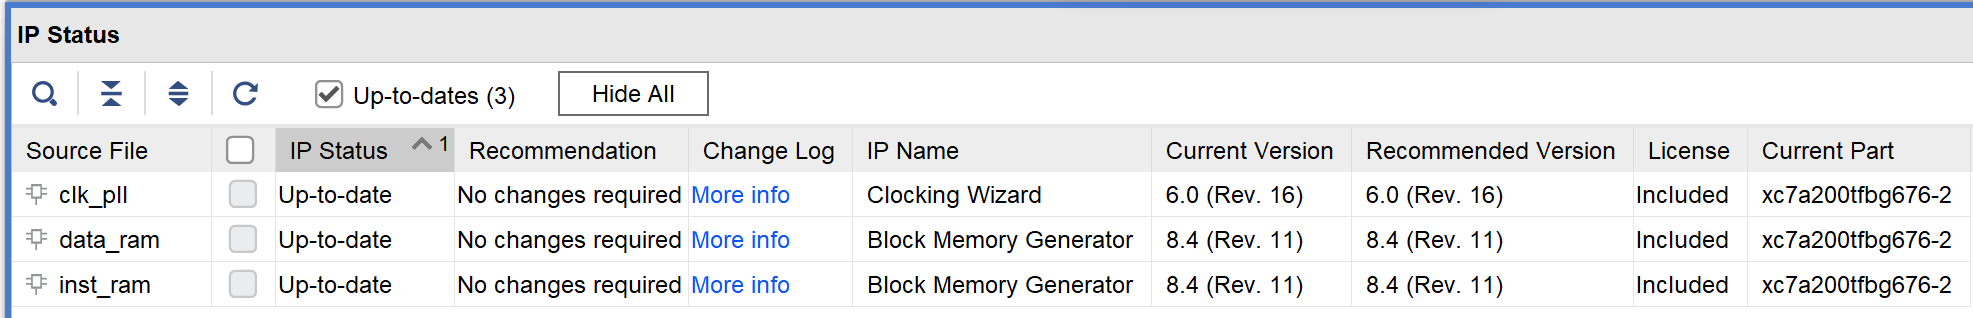
\includegraphics[width=0.8\linewidth]{fig/ip_update.png}
  \caption{升级后可正常工作的ip核}
  \label{fig:ip_update}
\end{figure}

\subsection{实践任务一：参考设计调试}
仿真时长设为 10\,ms。时钟周期是 10\,ns，为了报告的可读性和分析的方便，此处不直接使用 Vivado 仿真波形界面截图，而是选用 python matplotlib 读取每次仿真后保存的波形文件（.vcd、.wdb、.wcfg）进行可视化。
把 \texttt{clk} 画进全长图只会变成一条色带，所以图里只保留复位和写回比较用到的信号。修复前这些信号整段不变，每 5\,\textmu s 取一个点就够覆盖全貌；图宽 7.2\,inch、200\,dpi，大约一个像素对应 7\,\textmu s。后面每一处错误都只发生在报错前后的几拍，仍用同一组信号，但把时间轴缩到该次 \texttt{\$finish} 附近。

\subsubsection{BUG 1：译码级有效位没有赋值}
10\,ms 内 \texttt{debug\_wb\_pc}、写使能、写寄存器号和写数据始终是 X，\texttt{ds\_valid} 也是 X。\texttt{debug\_wb\_err} 一直为 0，因为 testbench 只在真正写非 0 寄存器时才和 \texttt{golden\_trace.txt} 比较。控制台从 22\,\textmu s 到 9.992\,ms 每 10\,\textmu s 重复同一行：
\begin{verbatim}
Test begin!
[  22000 ns] Test is running, debug_wb_pc = 0xxxxxxxxx
[9992000 ns] Test is running, debug_wb_pc = 0xxxxxxxxx
\end{verbatim}
\texttt{ds\_valid} 只有声明。它为 X 时 \texttt{ds\_allowin} 也为 X，取到的指令进不了译码级，写回级的 PC 寄存器始终没有被写入。按执行级、访存级同样的握手补上复位和更新：
\begin{verbatim}
if (reset)              ds_valid <= 1'b0;
else if (ds_allowin)    ds_valid <= fs_to_ds_valid;
\end{verbatim}
\begin{figure}[H]
  \centering
  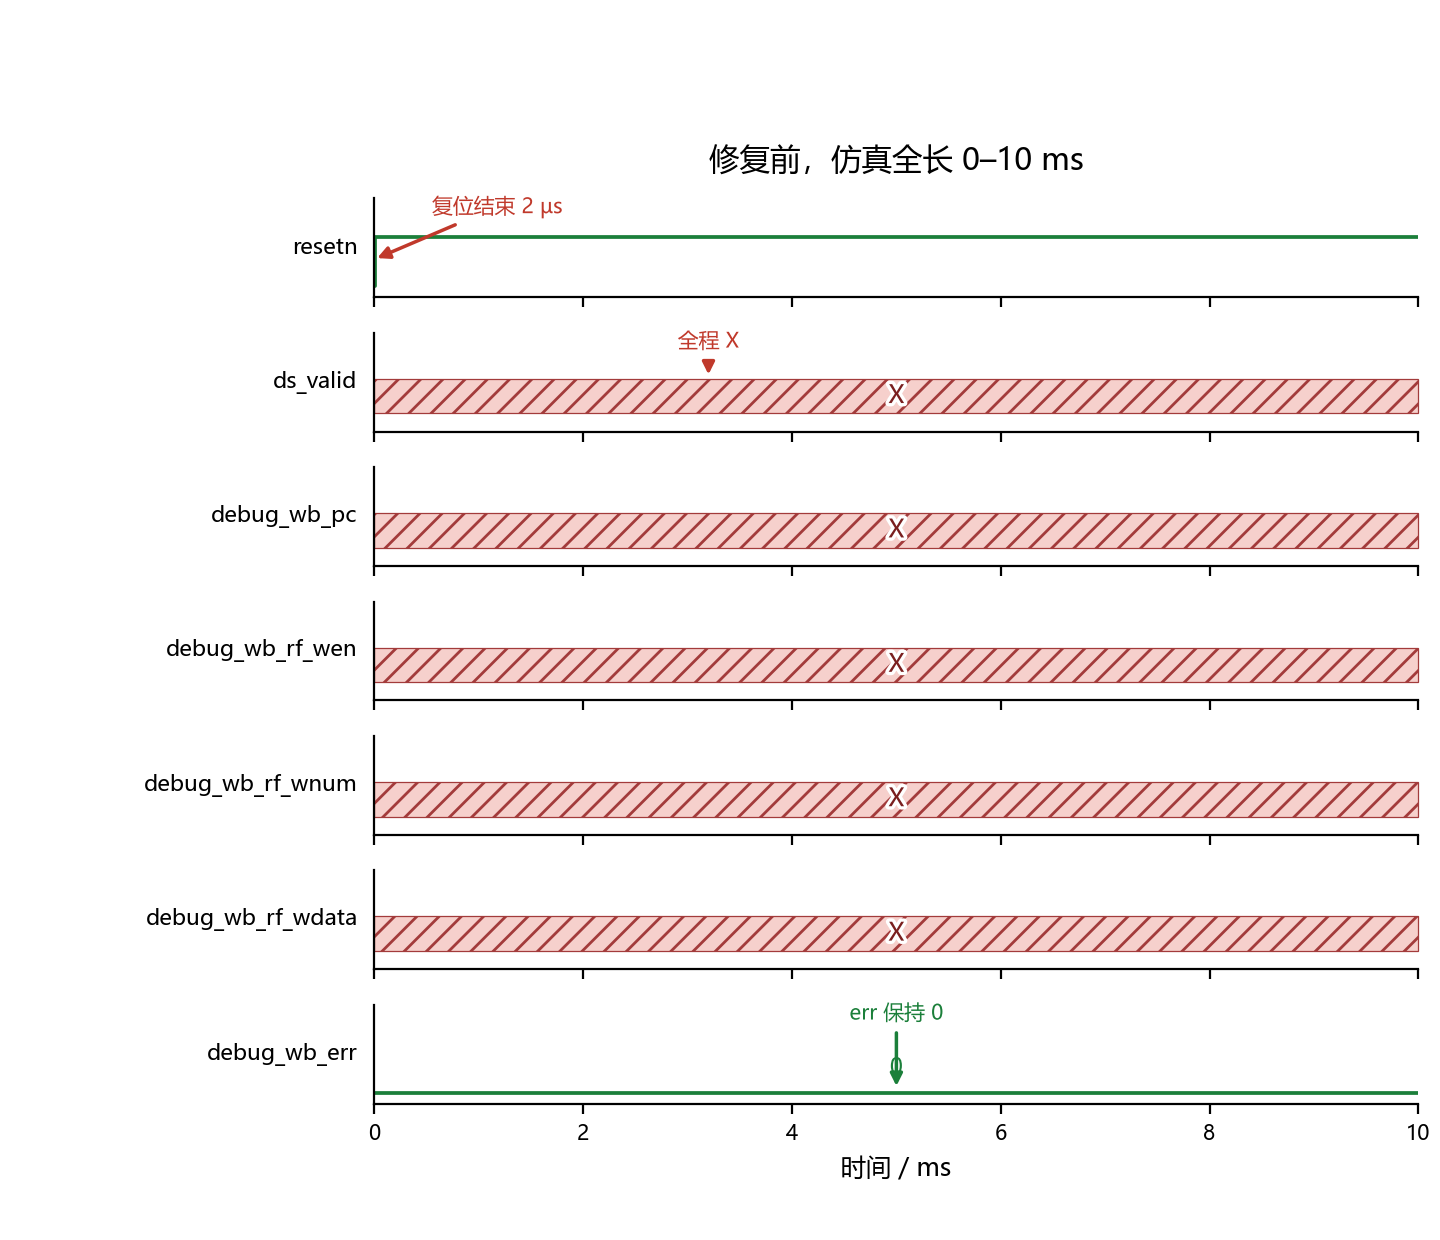
\includegraphics[width=\linewidth]{fig/bug1_10ms.png}
  \caption{修复前的 0--10\,ms。复位在 2\,\textmu s 结束，在这个尺度上只是左端一根线。}
\end{figure}

\subsubsection{BUG 2：\texttt{load\_op} 悬空}
补上 \texttt{ds\_valid} 后，第一条写回的 PC 和寄存器号已经正确，数据仍是 X。第一条指令是 \texttt{addiu \$8,\$0,-1}，参考数据为 \texttt{ffffffff}。
\begin{verbatim}
[2067 ns] Error!!!
reference: PC = 0xbfc00000, wb_rf_wnum = 0x08, wb_rf_wdata = 0xffffffff
mycpu    : PC = 0xbfc00000, wb_rf_wnum = 0x08, wb_rf_wdata = 0xxxxxxxxX
\end{verbatim}
总线上的 \texttt{load\_op} 从未赋值，执行级把它当作 \texttt{res\_from\_mem}。选择信号为 X 时，访存结果和 ALU 结果的二选一也是 X，算术指令同样写回 X。
\begin{verbatim}
assign load_op = inst_lw;
\end{verbatim}
\begin{figure}[H]
  \centering
  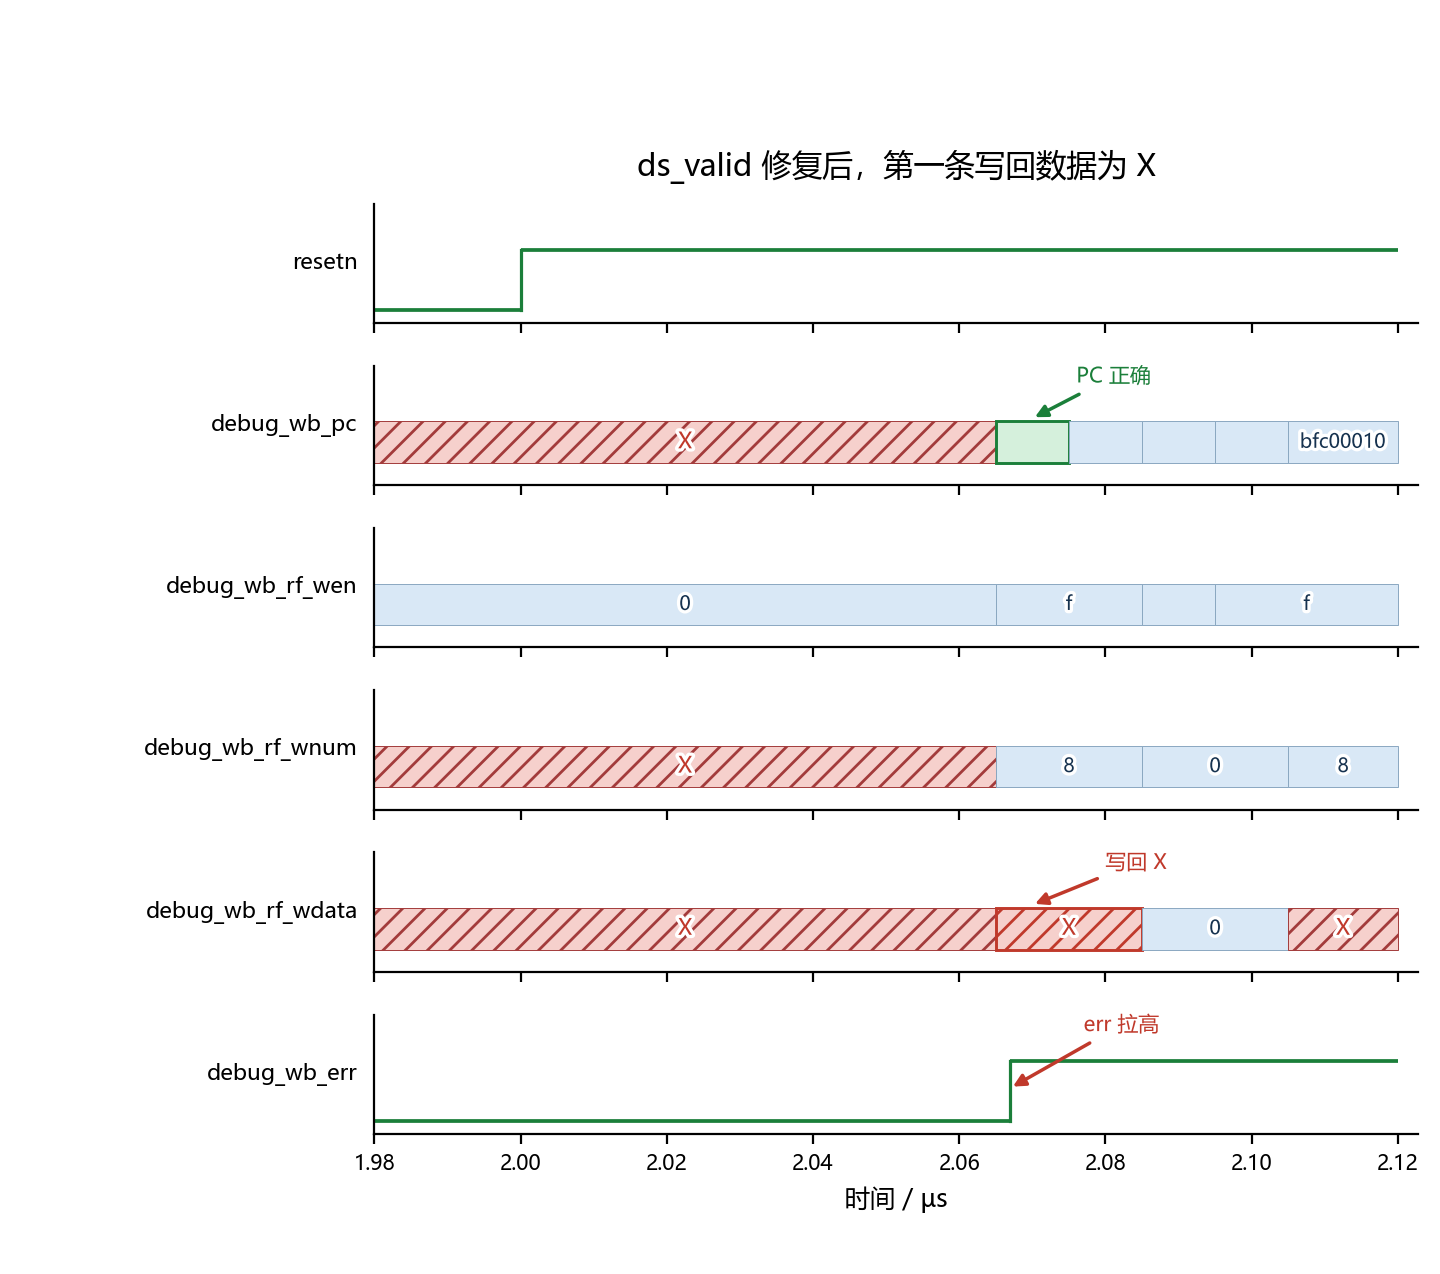
\includegraphics[width=\linewidth]{fig/bug2_wdata_x.png}
  \caption{2.065\,\textmu s 第一次写回：PC 与寄存器号正确，数据为 X，随后 \texttt{debug\_wb\_err} 拉高。}
\end{figure}

\subsubsection{BUG 3：ALU 的两个操作数都接到了 src2}
\texttt{load\_op} 接上之后，同一条 \texttt{addiu} 写出 \texttt{fffffffe}，而不是 \texttt{ffffffff}。立即数 \texttt{-1} 被加了两次。
\begin{verbatim}
[2067 ns] Error!!!
reference: PC = 0xbfc00000, wb_rf_wnum = 0x08, wb_rf_wdata = 0xffffffff
mycpu    : PC = 0xbfc00000, wb_rf_wnum = 0x08, wb_rf_wdata = 0xfffffffe
\end{verbatim}
\texttt{alu} 例化时 \texttt{alu\_src1} 和 \texttt{alu\_src2} 都接了 \texttt{es\_alu\_src2}。改为 \texttt{es\_alu\_src1}。
\begin{figure}[H]
  \centering
  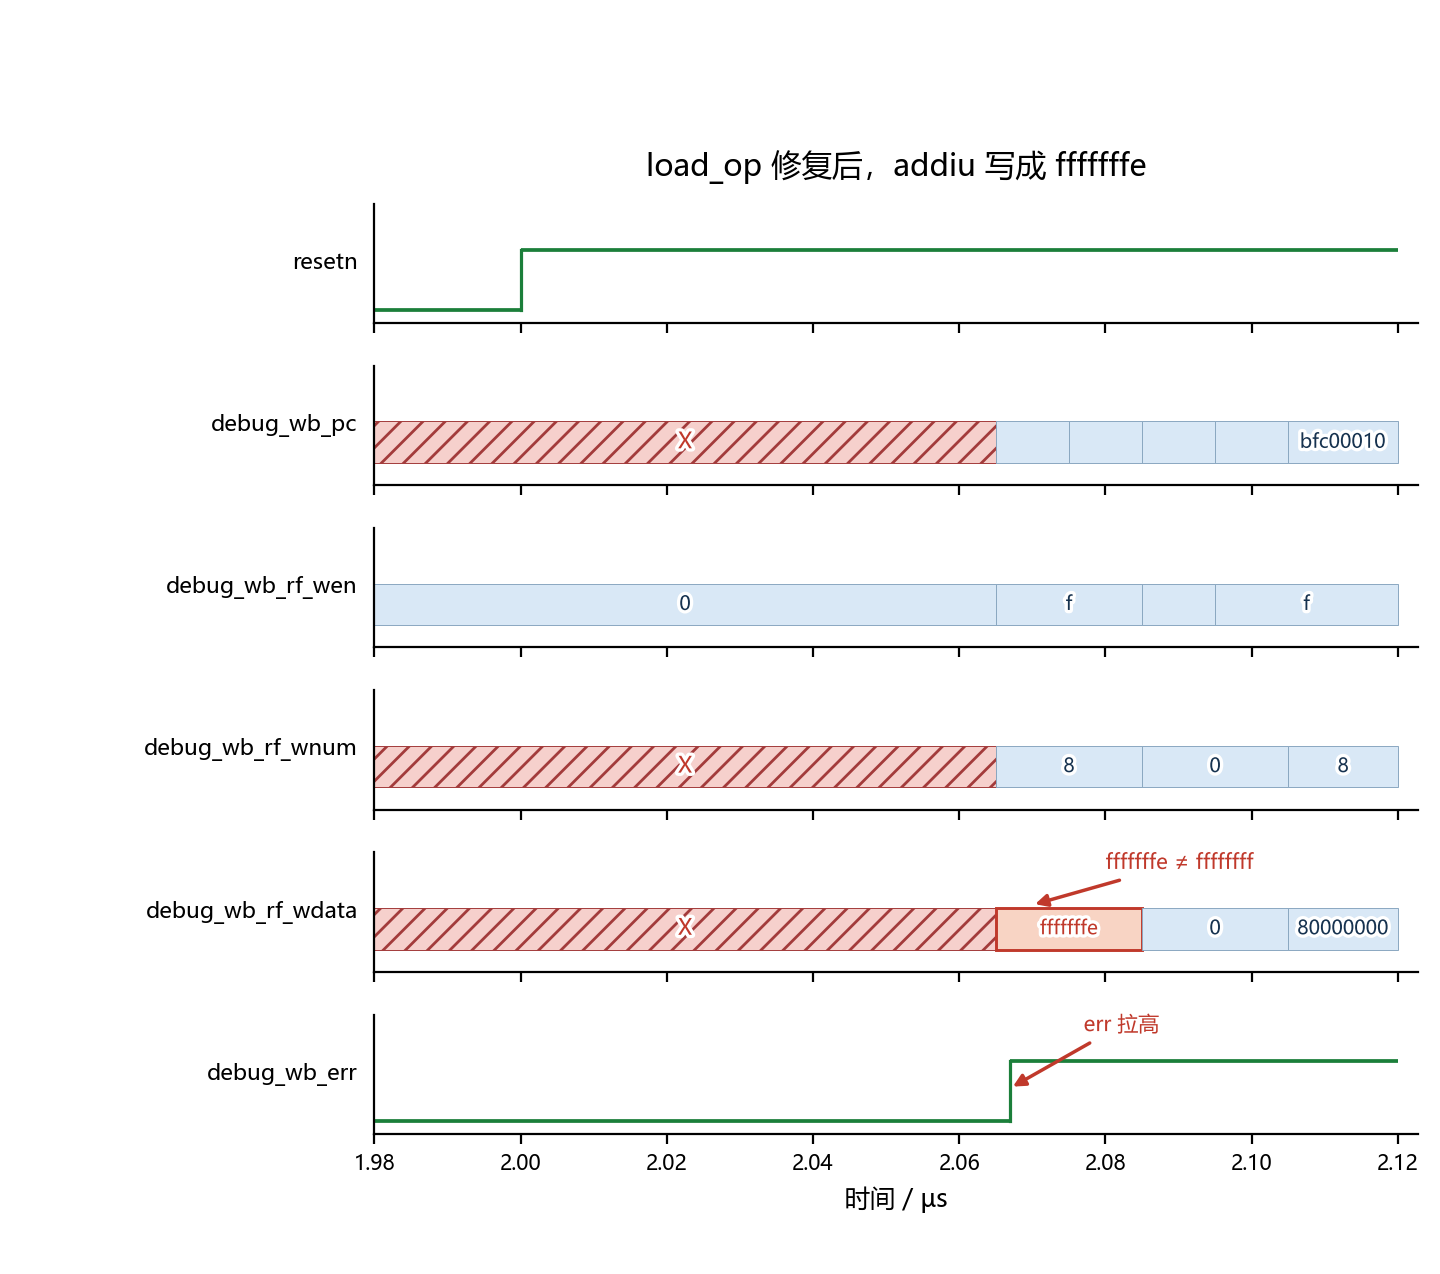
\includegraphics[width=\linewidth]{fig/bug3_addiu.png}
  \caption{复位后第一拍写回 \texttt{\$8}，数据为 \texttt{fffffffe}。}
\end{figure}

\subsubsection{BUG 4：分支总线少 1 位}
ALU 端口改对后，前两条 \texttt{addiu} 与参考轨迹一致，紧接着的 \texttt{beq \$0,\$0} 没有跳走。参考写回落在 \texttt{bfc0038c}，本设计继续顺序执行到 \texttt{bfc00010}。
\begin{verbatim}
[2107 ns] Error!!!
reference: PC = 0xbfc0038c, wb_rf_wnum = 0x04, wb_rf_wdata = 0xbfb00000
mycpu    : PC = 0xbfc00010, wb_rf_wnum = 0x08, wb_rf_wdata = 0x80000000
\end{verbatim}
\texttt{br\_bus} 是 \{\texttt{br\_taken}, \texttt{br\_target}\}，共 33 位，而 \texttt{BR\_BUS\_WD} 定义为 32，\texttt{br\_taken} 被截掉。改为 33 之后这条 \texttt{beq} 能跳到 \texttt{bfc0038c}。本测试程序里跳转基址用 IF 级的 \texttt{fs\_pc}，在顺序取指时它正好是延迟槽的 PC，与参考轨迹一致，因此没有改目标地址的计算公式。
\begin{figure}[H]
  \centering
  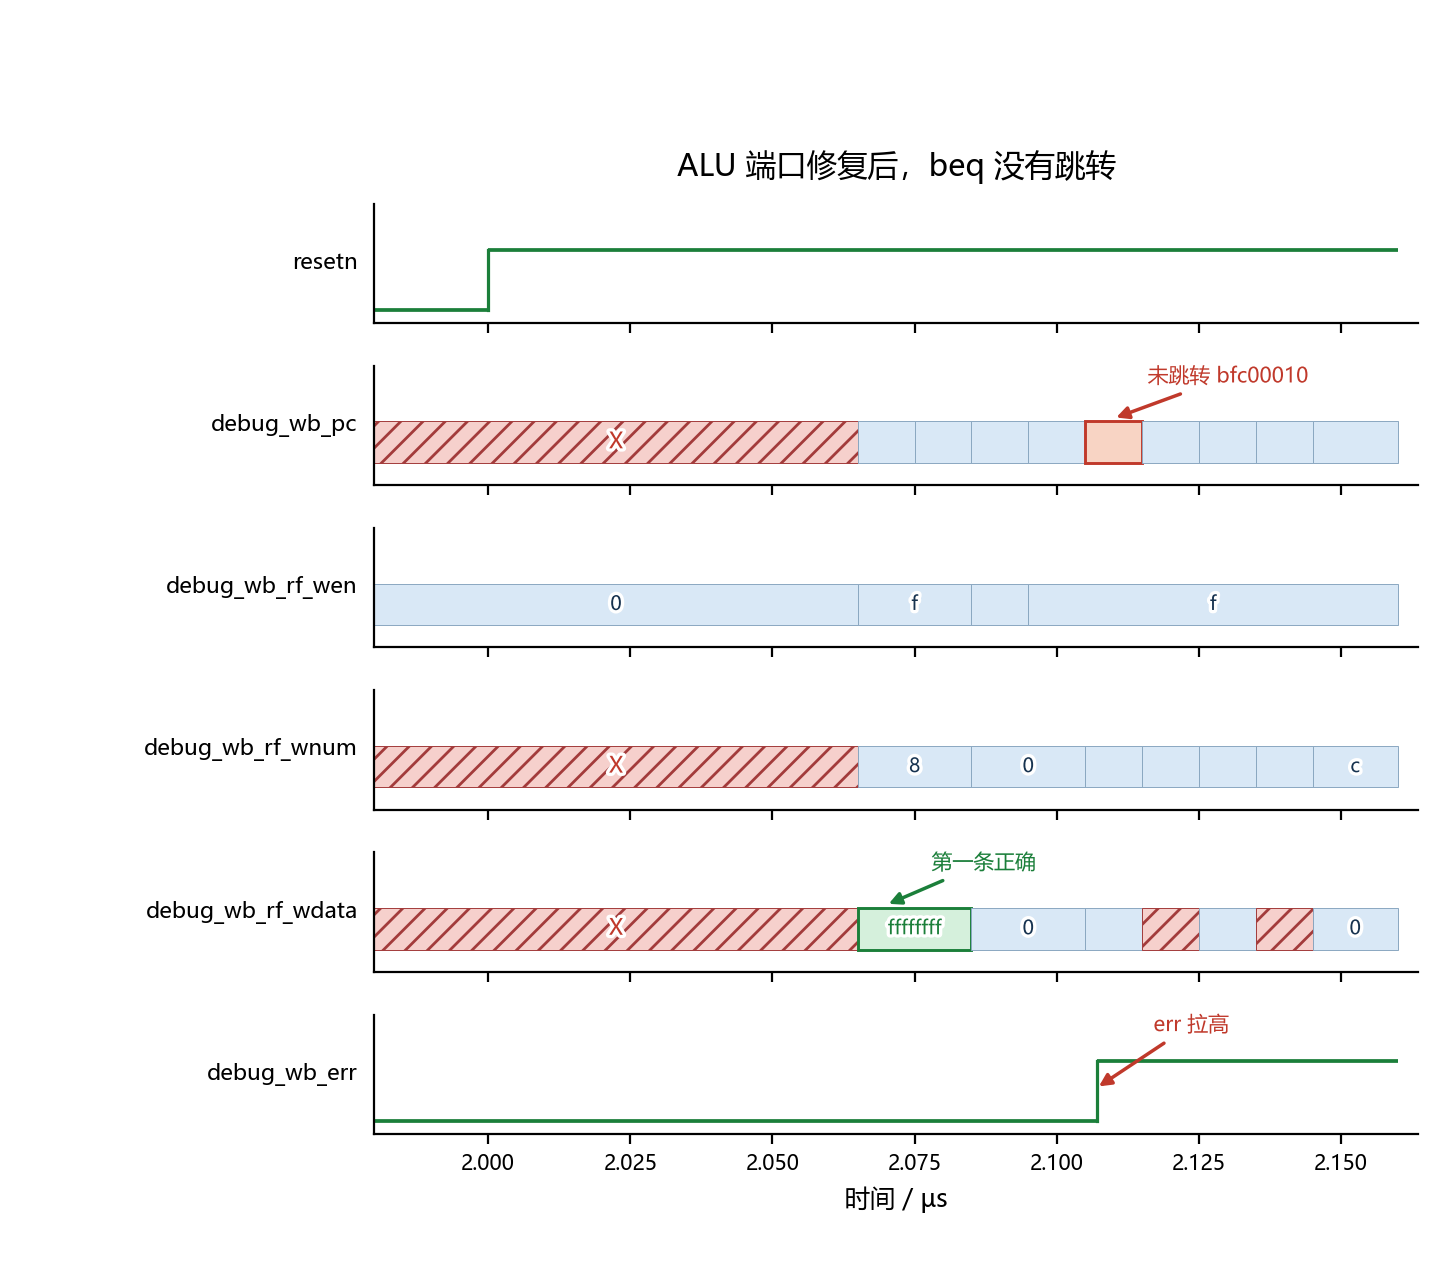
\includegraphics[width=\linewidth]{fig/bug4_branch.png}
  \caption{第一条 \texttt{addiu} 已写成 \texttt{ffffffff}，随后 PC 仍沿 \texttt{bfc00010} 顺序前进。}
\end{figure}

\subsubsection{BUG 5：逻辑右移丢掉最高位}
分支总线加宽后，功能点 01 到 11 通过，12 号 \texttt{srl} 失败。PC 和寄存器号与参考相同，数据只差最高位：\texttt{adff20c0} 变成 \texttt{2dff20c0}。
\begin{verbatim}
[888537 ns] Error!!!
reference: PC = 0xbfc88c90, wb_rf_wnum = 0x02, wb_rf_wdata = 0xadff20c0
mycpu    : PC = 0xbfc88c90, wb_rf_wnum = 0x02, wb_rf_wdata = 0x2dff20c0
\end{verbatim}
\texttt{sr\_result} 取了 \texttt{sr64\_result[30:0]}，32 位结果的最高位被补成 0。改为 \texttt{[31:0]}。
\begin{figure}[H]
  \centering
  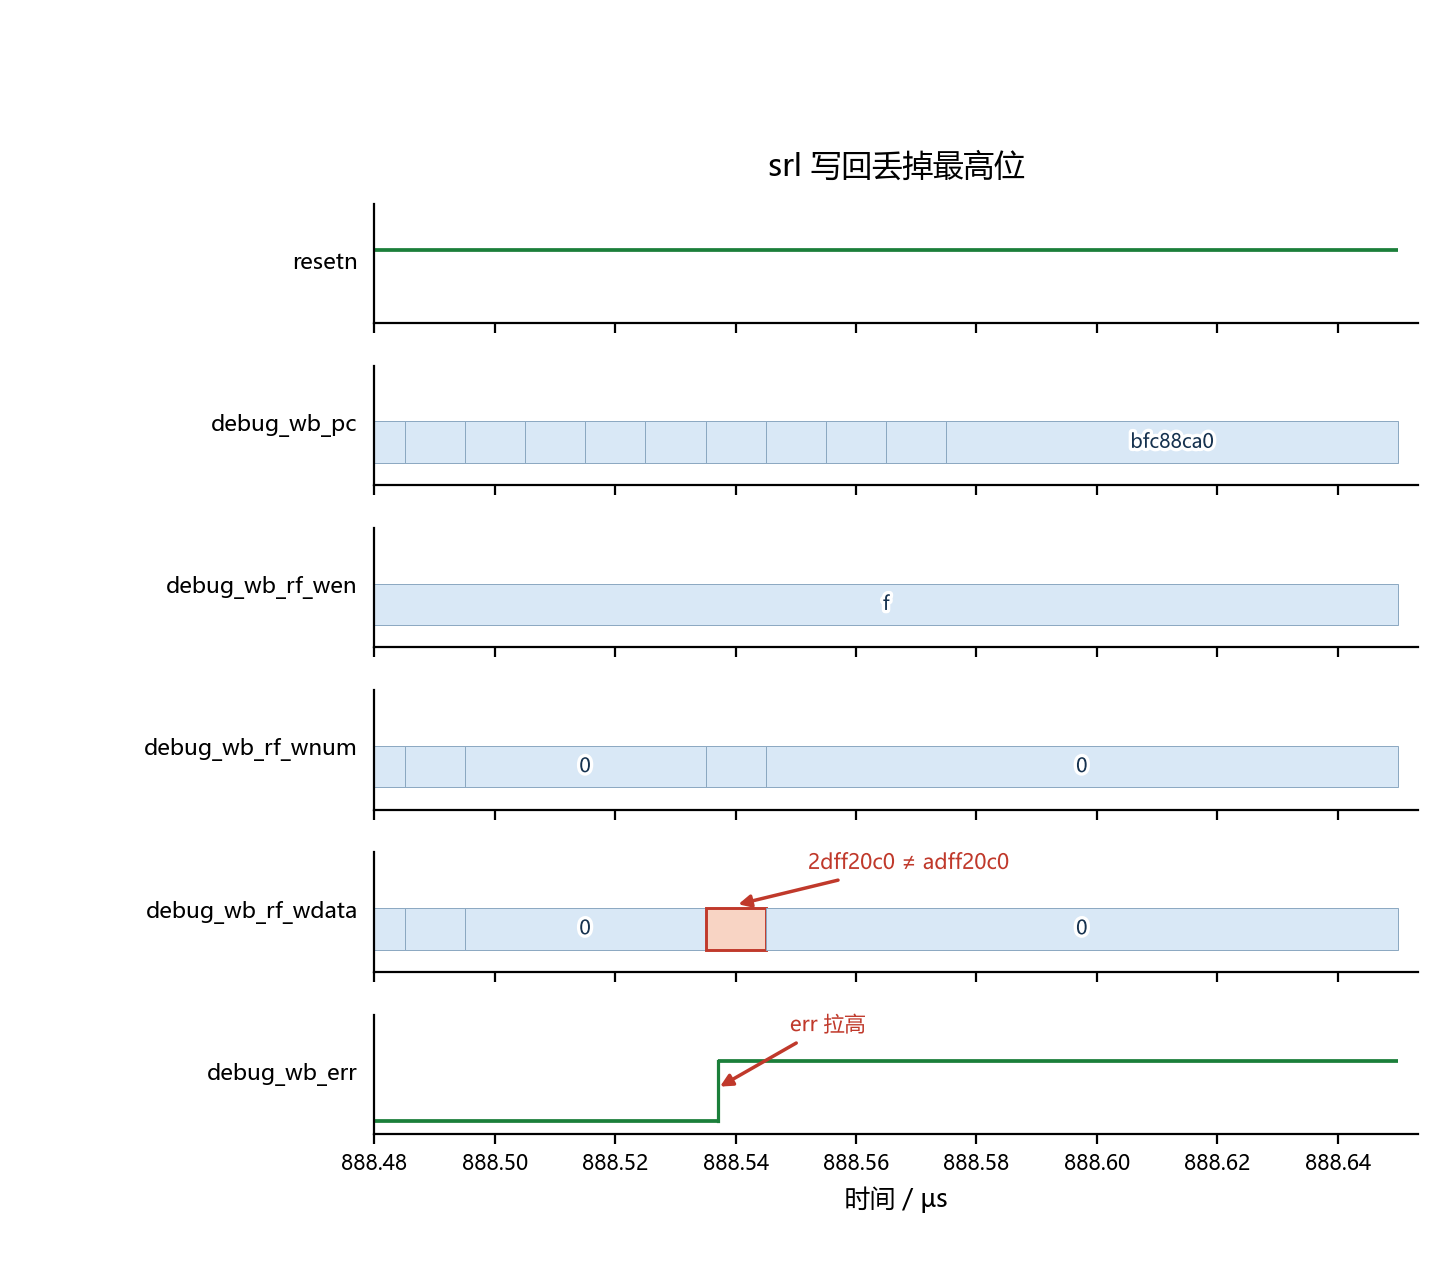
\includegraphics[width=\linewidth]{fig/bug5_srl.png}
  \caption{888.54\,\textmu s 附近 \texttt{\$2} 写成 \texttt{2dff20c0}，\texttt{debug\_wb\_err} 随之拉高。}
\end{figure}

\subsubsection{BUG 6：\texttt{or} 结果回或了自身}
\texttt{alu.v} 中原来写着
\begin{verbatim}
assign or_result = alu_src1 | alu_src2 | alu_result;
\end{verbatim}
\texttt{alu\_result} 又由 \texttt{or\_result} 组合出来，形成组合环。把这条自反馈去掉之后，08 号 \texttt{or} 功能点通过。把自反馈暂时加回去再仿真，08 号功能点仍然 PASS：xsim 把环收敛到了 \texttt{src1|src2}。轨迹没有单独报这一处，但组合环不能留在电路里，最终版本是
\begin{verbatim}
assign or_result = alu_src1 | alu_src2;
\end{verbatim}

\subsubsection{BUG 7：访存级使用阻塞赋值}
\texttt{MEM\_stage.v} 在时钟过程里用 \texttt{es\_to\_ms\_bus\_r = es\_to\_ms\_bus}。\texttt{lw}/\texttt{sw} 功能点在本机 xsim 上仍然通过，因为进程调度碰巧让写回采到了正确数据。这和其它级的非阻塞赋值不一致，换仿真器时可能在同一拍读到新值。改为 \texttt{<=}。

\texttt{decoder\_6\_64} 的循环上界原来是 63，\texttt{out[63]} 悬空。\texttt{func\_lab3} 用不到操作码或功能码 63，一并把上界改为 64。

上述修改全部保留后重新仿真，23 个功能点通过，测试在 1.728\,ms 结束，没有再跑满 10\,ms。控制台末尾为：
\begin{verbatim}
----[1726905 ns] Number 8'd23 Functional Test Point PASS!!!
Test end!
----PASS!!!
$finish called at time : 1728025 ns
\end{verbatim}
\begin{figure}[H]
  \centering
  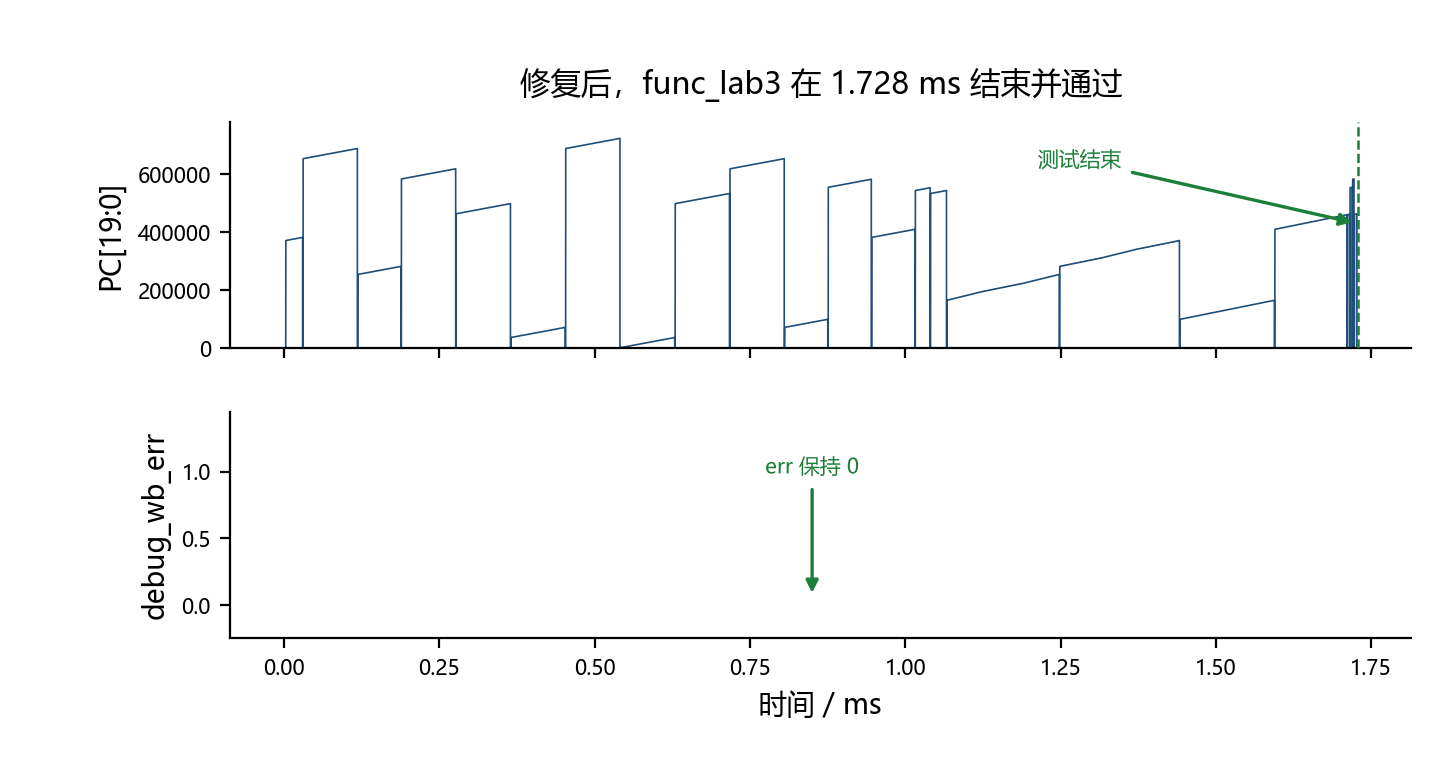
\includegraphics[width=\linewidth]{fig/pass_10ms.png}
  \caption{修复后的全程。纵轴是写回 PC 的低 20 位，\texttt{debug\_wb\_err} 保持 0，直到测试结束。}
\end{figure}

\begin{table}[H]
  \centering
  \caption{任务一 bug 记录}
  \begin{tabular}{clp{7.4cm}}
    \toprule
    编号 & 位置 & 现象与改法 \\
    \midrule
    1 & \texttt{ID\_stage.v} & \texttt{ds\_valid} 未赋值，10\,ms 内 PC 为 X。补复位和更新。 \\
    2 & \texttt{ID\_stage.v} & \texttt{load\_op} 悬空，写回数据为 X。接到 \texttt{inst\_lw}。 \\
    3 & \texttt{EXE\_stage.v} & ALU 两个输入都是 src2，\texttt{addiu} 得到 \texttt{fffffffe}。 \\
    4 & \texttt{mycpu.h} & \texttt{BR\_BUS\_WD} 为 32，分支不发生。改为 33。 \\
    5 & \texttt{alu.v} & 右移结果取 \texttt{[30:0]}，最高位丢失。改为 \texttt{[31:0]}。 \\
    6 & \texttt{alu.v} & \texttt{or} 回或 \texttt{alu\_result}。去掉自反馈。 \\
    7 & \texttt{MEM\_stage.v} & 总线寄存使用阻塞赋值。改为非阻塞赋值。 \\
    \bottomrule
  \end{tabular}
\end{table}


\subsection{实践任务二：阻塞}
任务一用的 \texttt{func\_lab3} 在相关指令之间插入了 4 条 \texttt{addu \$0,\$0,\$0}，消费者落到写回之后才进入译码级，看不出写后读。
\texttt{func\_lab4} 把 \texttt{NOP} 宏改成空，\texttt{LI} 里只留下 3 条 \texttt{nop}。把 \texttt{inst\_ram} 换成
\texttt{soft/func\_lab4/obj/inst\_ram.coe}，用 \texttt{cpu132\_gettrace} 重新生成 \texttt{golden\_trace.txt}。
参考轨迹在 1.184\,ms 结束。

\subsubsection{未加阻塞时的写后读}
寄存器堆在写回级的时钟沿写入，译码级组合读出。生产者还在 EX、MEM 或 WB 时，译码级读到的是旧值；若该寄存器从未写过，仿真里就是 X。
\texttt{start.S} 里 \texttt{lui \$s0, 0} 之后只有 \texttt{jal n1\_lui\_test} 和延迟槽，测试入口第一条就是 \texttt{addiu \$s0, \$s0, 1}。
当这条 \texttt{addiu} 停在 ID 时，\texttt{lui \$s0} 正好在 WB，同拍读到 X。

\begin{verbatim}
[2537 ns] Error!!!
reference: PC = 0xbfc408b0, wb_rf_wnum = 0x10, wb_rf_wdata = 0x00000001
mycpu    : PC = 0xbfc408b0, wb_rf_wnum = 0x10, wb_rf_wdata = 0xxxxxxxxx
\end{verbatim}

\begin{figure}[H]
  \centering
  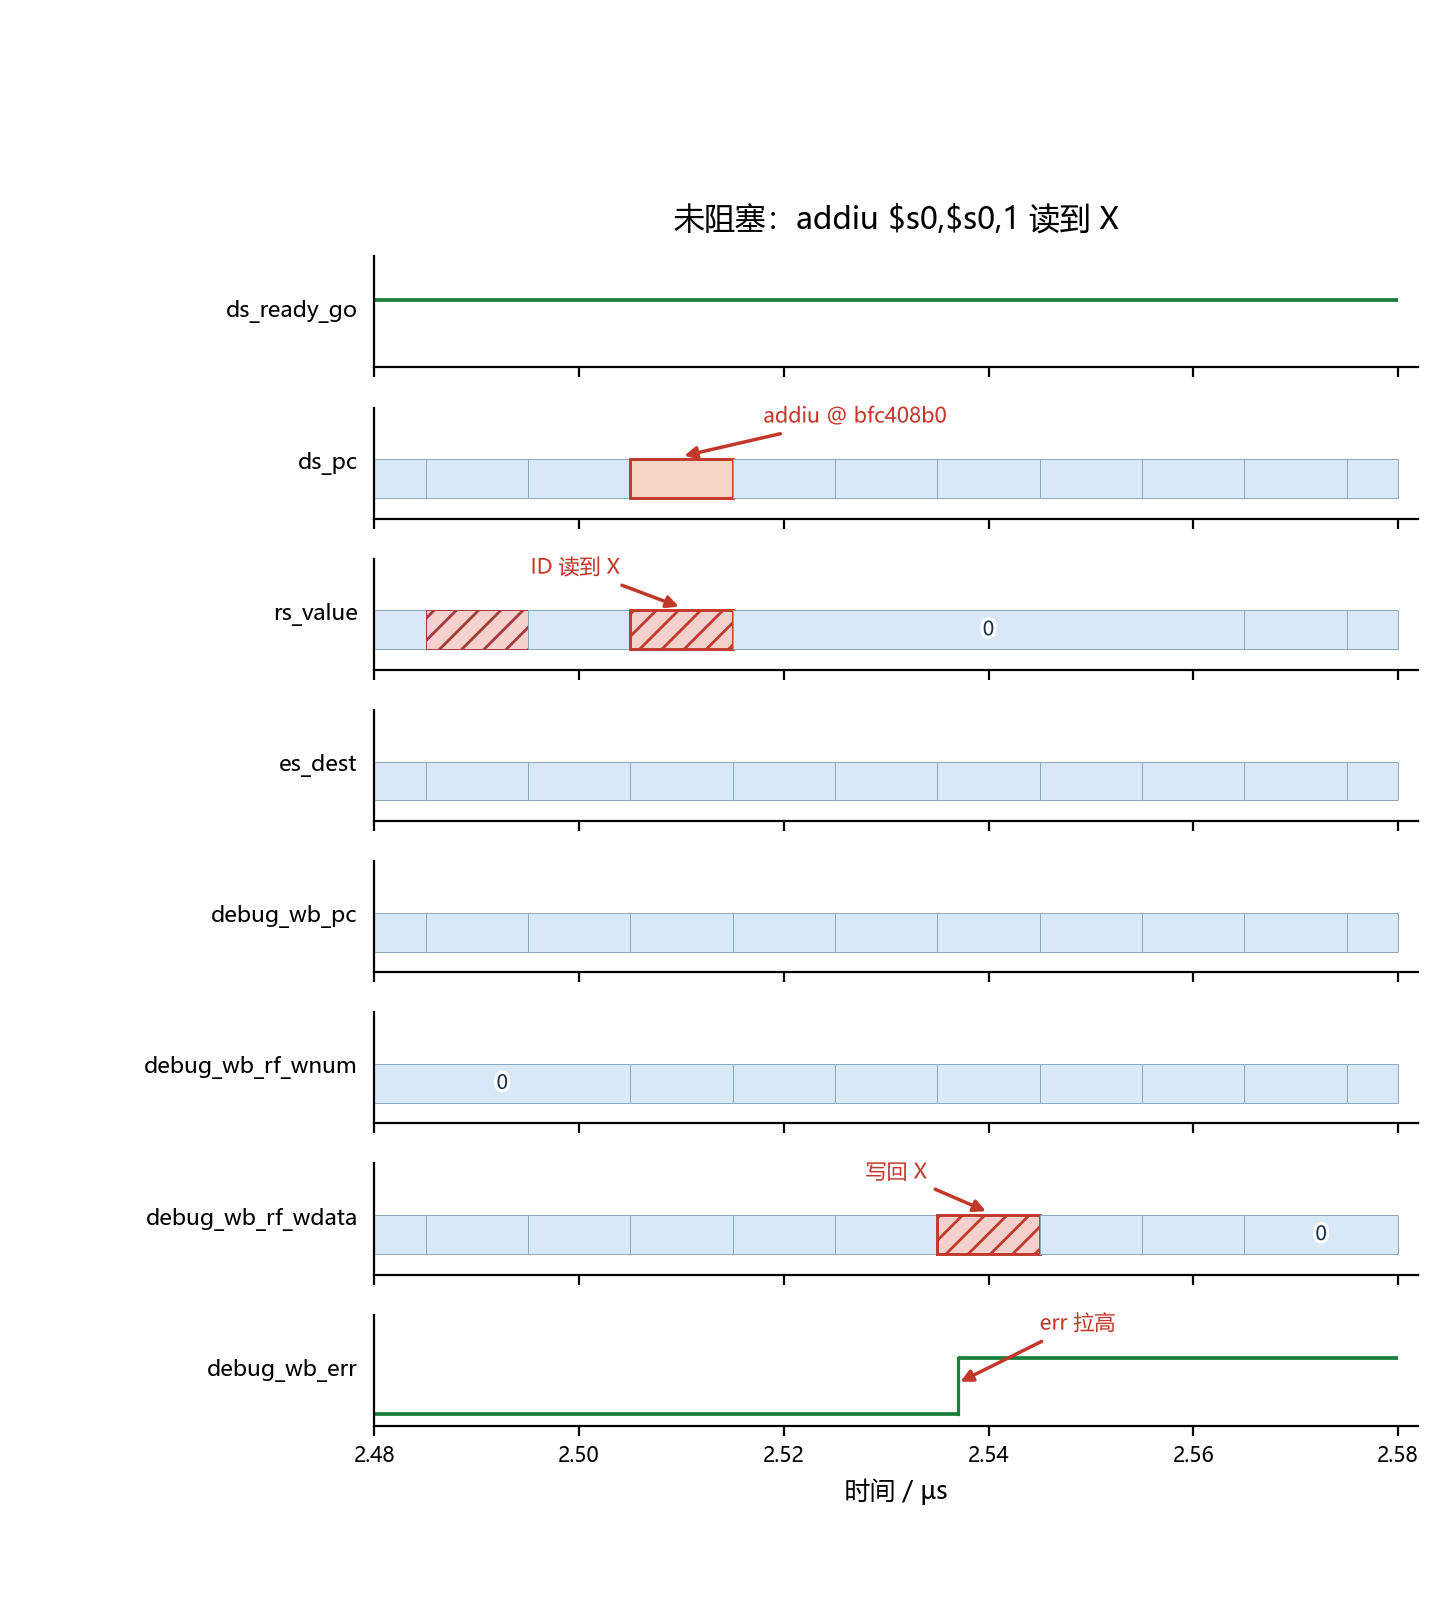
\includegraphics[width=\linewidth]{fig/stall_before.png}
  \caption{未阻塞。\texttt{ds\_pc=bfc408b0} 的 \texttt{addiu \$s0,\$s0,1} 在 ID 时 \texttt{rs\_value} 为 X，
  随后写回 X，\texttt{debug\_wb\_err} 拉高。}
  \label{fig:stall-before}
\end{figure}

\subsubsection{阻塞逻辑}
译码级根据本条是否使用 \texttt{rs}/\texttt{rt}，与 EX、MEM、WB 的写目的比较。命中且目的不是 \texttt{\$0} 时，
\texttt{ds\_ready\_go=0}：IF 因 \texttt{ds\_allowin} 为低而停住，进入 EX 的 \texttt{valid} 为低，形成气泡。
写回与译码同拍时寄存器堆仍是旧值，因此 WB 命中也停一拍，下一拍再读。阻塞期间把 \texttt{br\_taken} 拉低，避免用旧比较结果改 PC。

\begin{verbatim}
assign ds_ready_go = ~(es_raw | ms_raw | ws_raw);
assign br_taken    = (...分支条件...) && ds_valid && ds_ready_go;
\end{verbatim}

EX、MEM 的 \texttt{valid}、\texttt{gr\_we}、\texttt{dest} 送到 ID；WB 用已有的 \texttt{ws\_to\_rf\_bus} 里的 \texttt{rf\_we}/\texttt{rf\_waddr}。

\begin{figure}[H]
  \centering
  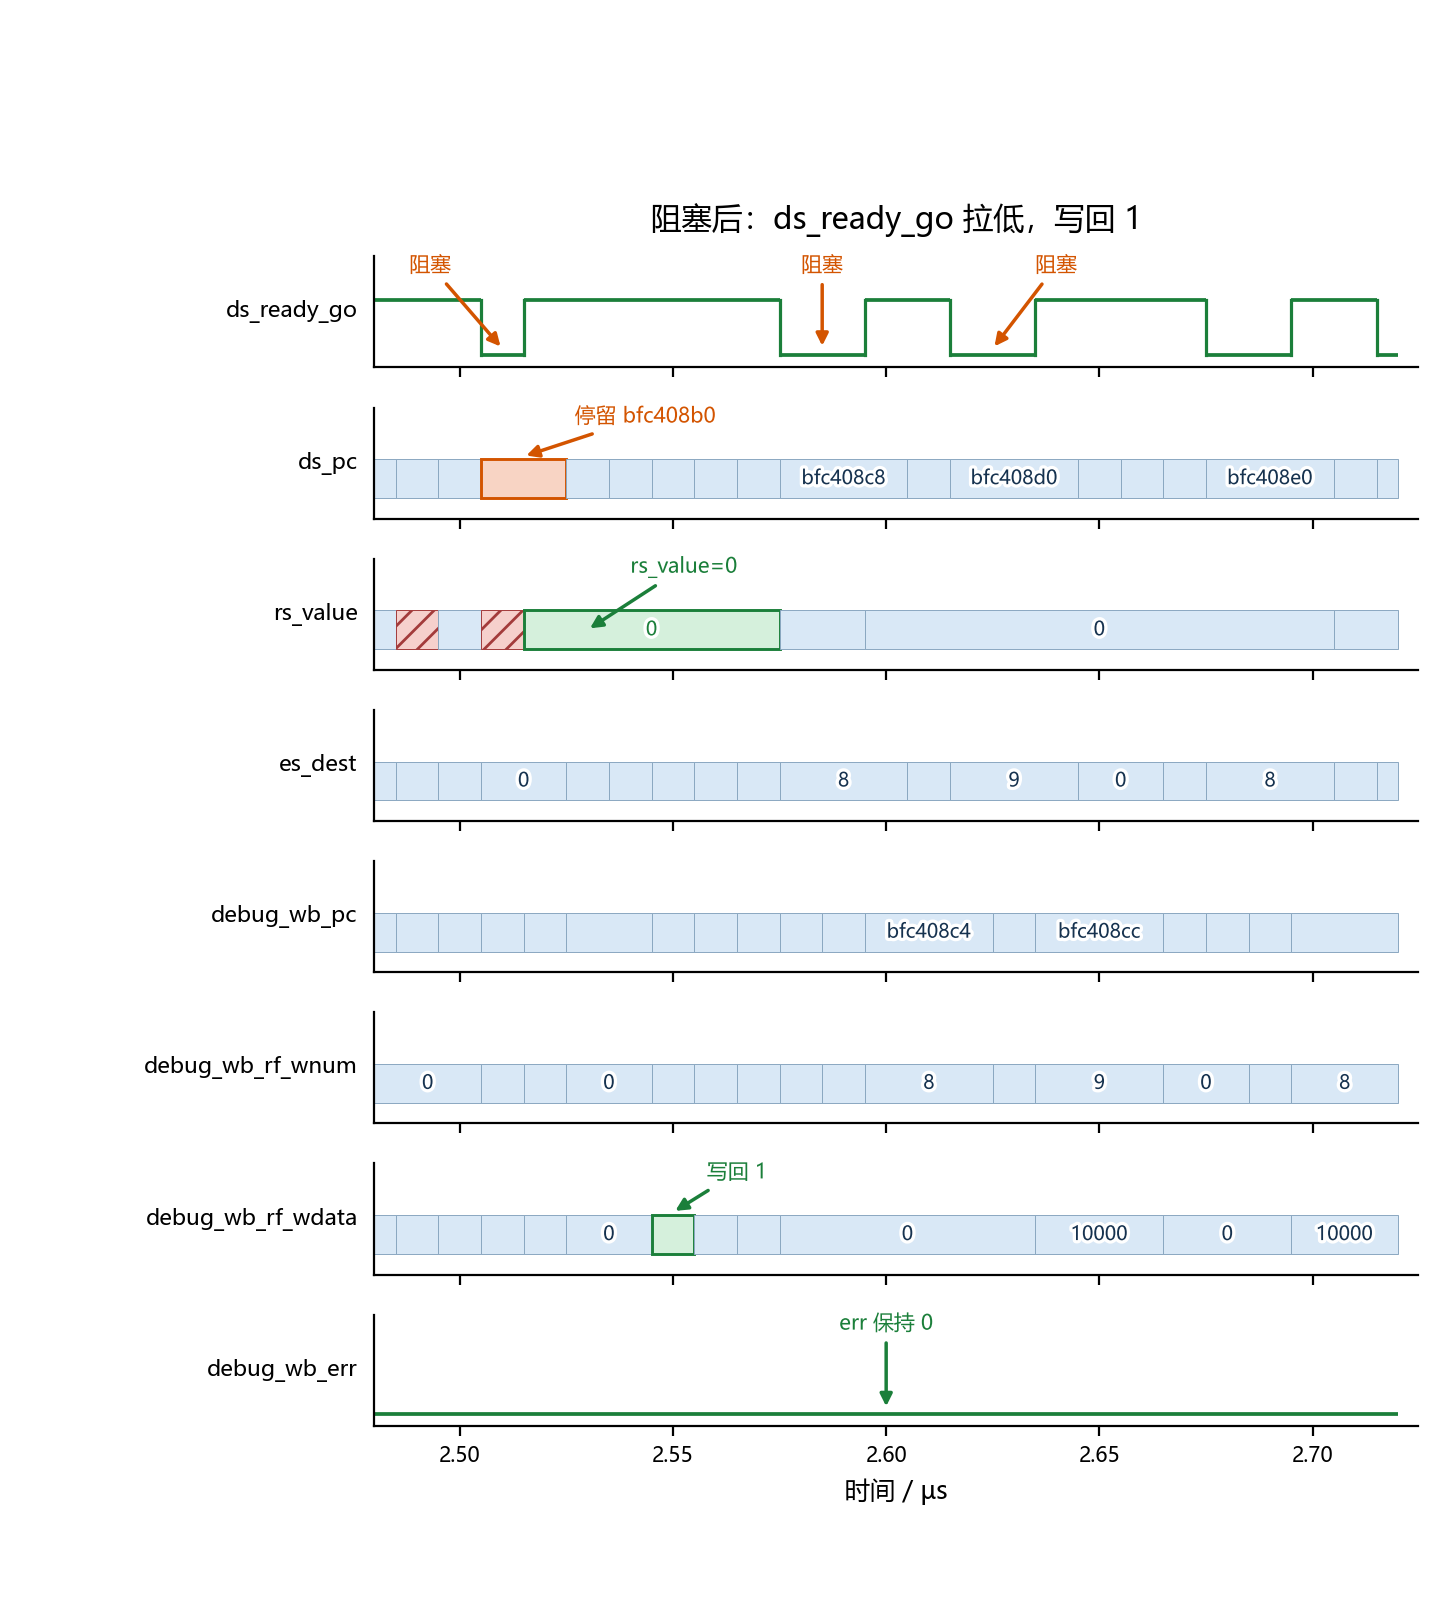
\includegraphics[width=\linewidth]{fig/stall_after.png}
  \caption{阻塞后同一段。\texttt{ds\_ready\_go} 多次拉低，\texttt{ds\_pc} 在 \texttt{bfc408b0} 停留，
  \texttt{rs\_value} 变为 0 后再放行。\texttt{debug\_wb\_err} 保持 0。}
  \label{fig:stall-after}
\end{figure}

加阻塞后 23 个功能点全部通过，测试在 1.311\,ms 结束，比参考 CPU 的 1.184\,ms 多出约 $1.27\times10^{4}$ 个时钟（周期 10\,ns）。多出来的就是气泡。控制台末尾：
\begin{verbatim}
----[1310005 ns] Number 8'd23 Functional Test Point PASS!!!
Test end!
----PASS!!!
$finish called at time : 1310945 ns
\end{verbatim}


\subsection{实践任务三：前递}
在阻塞版本上增加旁路。ALU 相关不再插入气泡；load 在 EX、消费者已在 ID 时仍停一拍。
与任务二使用同一段 \texttt{hmc\_lab4} 程序。

阻塞时 EX、MEM、WB 命中都把 \texttt{ds\_ready\_go} 拉低。前递把尚未写回的结果接到译码级的 \texttt{rs\_value}/\texttt{rt\_value}，优先级 EX $>$ MEM $>$ WB $>$ 寄存器堆。分支比较和 \texttt{jr} 用的也是这两个值。只保留 load-use：生产者是 \texttt{lw} 且还在 EX 时停一拍，下一拍从 MEM 前递 \texttt{ms\_final\_result}。

任务二里 \texttt{lui \$s0, 0} 与 \texttt{addiu \$s0, \$s0, 1} 隔着 \texttt{jal} 和延迟槽。加前递后 2.505\,\textmu s \texttt{addiu} 进入 ID 时 \texttt{ds\_ready\_go} 保持 1，\texttt{rs\_value} 取自 WB 的 0，不再插入气泡。相邻 ALU 相关更清楚的是 \texttt{n2\_addu} 里 \texttt{addu \$v0, \$t0, \$t1} 紧跟 \texttt{bne \$v0, \$v1}：14.755\,\textmu s \texttt{bne} 在 ID、\texttt{addu} 在 EX，\texttt{rs\_value} 与 \texttt{es\_alu\_result} 同为 \texttt{6cbc4bde}，没有气泡。见图~\ref{fig:fwd-ex}。

\begin{figure}[H]
  \centering
  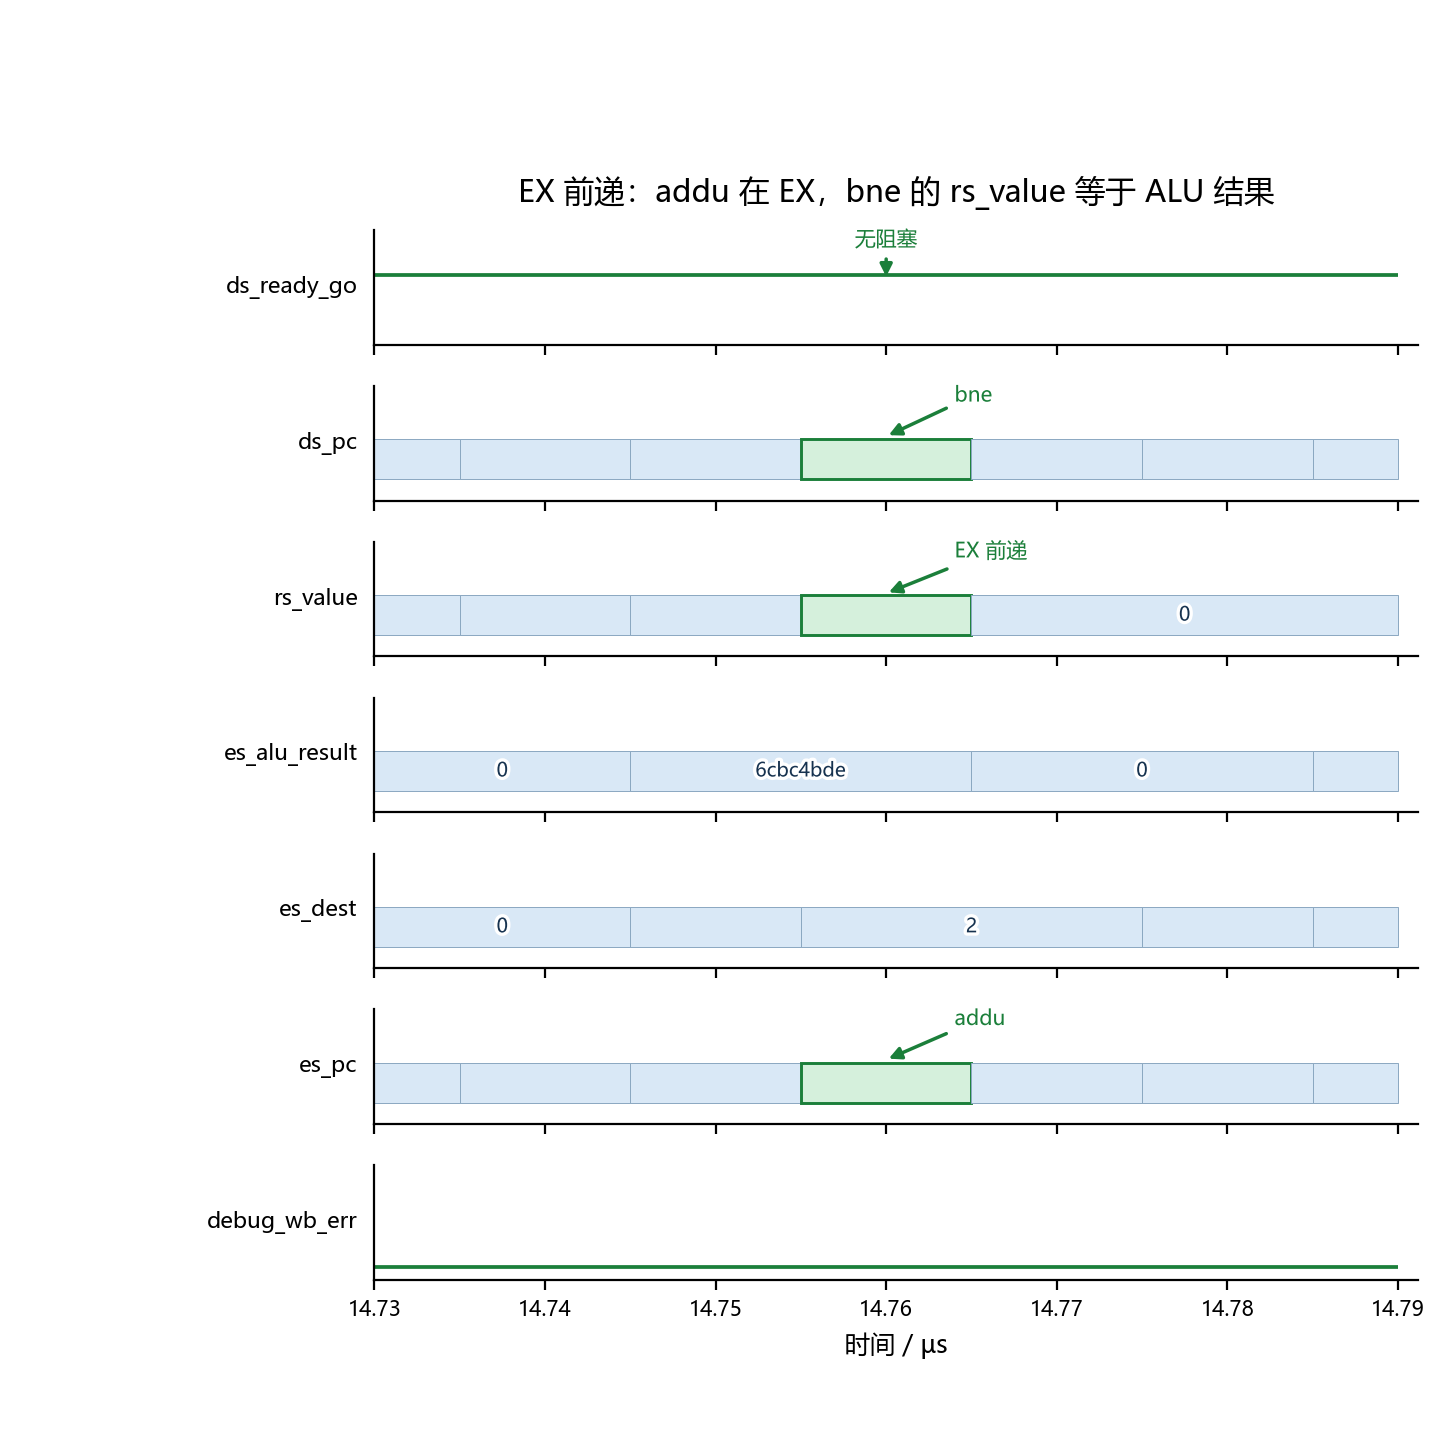
\includegraphics[width=\linewidth]{fig/fwd_ex.png}
  \caption{14.75\,\textmu s 附近。\texttt{ds\_pc=bfc6de28} 的 \texttt{bne} 在 ID，
  \texttt{es\_pc=bfc6de24} 的 \texttt{addu} 在 EX，\texttt{rs\_value} 等于 ALU 结果，
  \texttt{ds\_ready\_go} 保持 1。}
  \label{fig:fwd-ex}
\end{figure}

\texttt{TEST\_LW} 的四条 \texttt{lw} 之后仍隔着比较，真正相邻的 load-use 在 \texttt{wait\_1s}：
\texttt{lw \$t2, 0(\$t0)} 紧跟 \texttt{xor \$t2, \$t2, \$t1}。
14.385\,\textmu s \texttt{xor} 进入 ID 时 load 还在 EX，\texttt{es\_load\_op=1}，\texttt{ds\_ready\_go} 拉低一拍，EX 出现气泡；
下一拍 load 已到 MEM，\texttt{rs\_value} 与 \texttt{ms\_final\_result} 同为 \texttt{aaaa}，再放行。见图~\ref{fig:fwd-load}。

\begin{figure}[H]
  \centering
  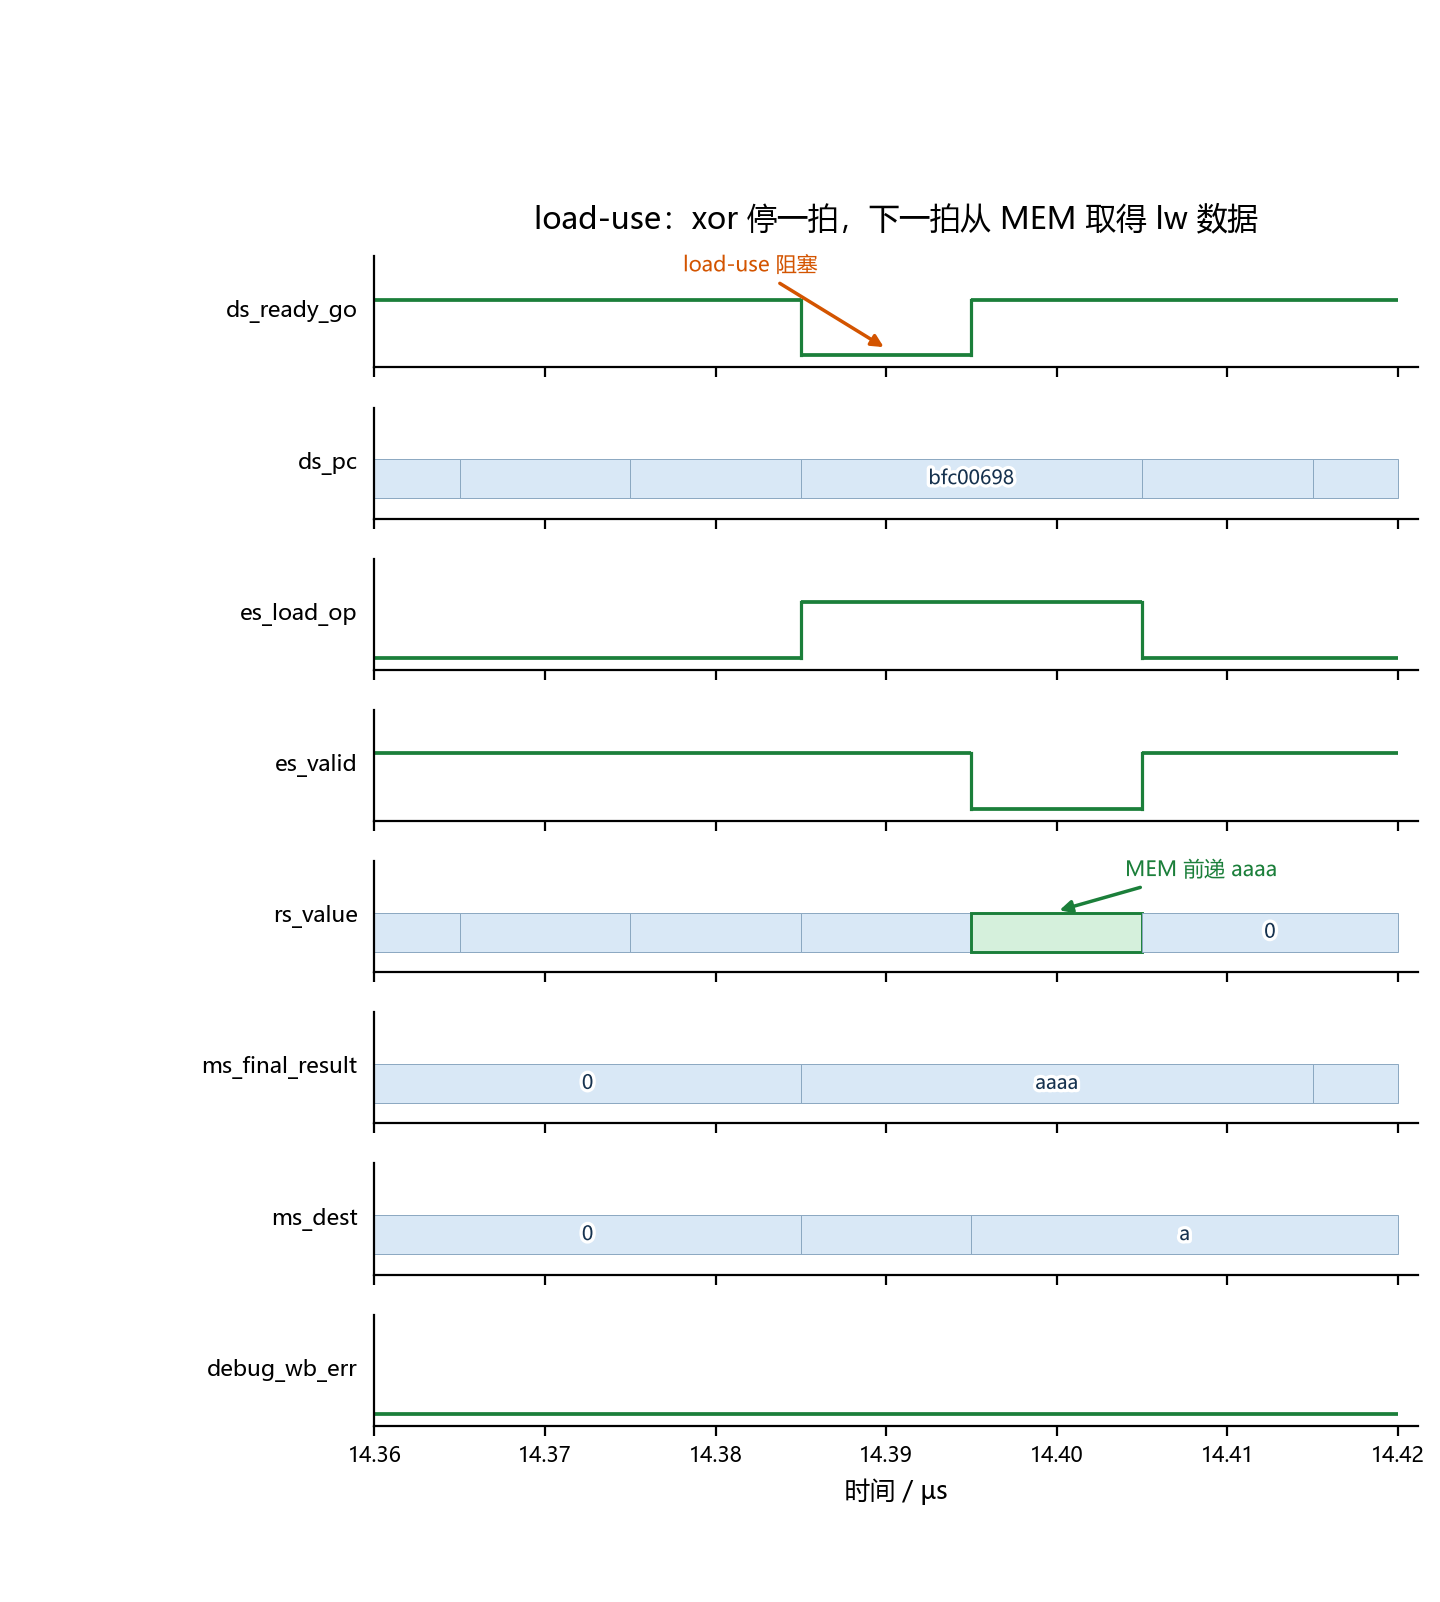
\includegraphics[width=\linewidth]{fig/fwd_load.png}
  \caption{14.39\,\textmu s 附近。\texttt{ds\_pc} 在 \texttt{bfc00698} 停留一拍，
  随后 \texttt{rs\_value} 变成访存结果。}
  \label{fig:fwd-load}
\end{figure}

加前递后 23 个功能点全部通过，测试在 1.148\,ms 结束，短于阻塞的 1.311\,ms，并略短于参考 CPU 的 1.184\,ms，比阻塞少约 $1.63\times 10^{4}$ 拍。控制台末尾：
\begin{verbatim}
----[1147165 ns] Number 8'd23 Functional Test Point PASS!!!
Test end!
----PASS!!!
$finish called at time : 1147805 ns
\end{verbatim}

\section{关键代码}
任务一里改过的赋值、端口和总线宽度已经写在上一节。下面留给阻塞和前递。

\subsection{译码级阻塞}
\begin{verbatim}
wire rs_need = inst_addu | inst_subu | inst_slt | inst_sltu
             | inst_and  | inst_or   | inst_xor | inst_nor
             | inst_addiu| inst_lw   | inst_sw  | inst_beq
             | inst_bne  | inst_jr;
wire rt_need = inst_addu | inst_subu | inst_slt | inst_sltu
             | inst_and  | inst_or   | inst_xor | inst_nor
             | inst_sll  | inst_srl  | inst_sra | inst_sw
             | inst_beq  | inst_bne;
wire es_raw = es_valid && es_gr_we && (es_dest != 5'd0) &&
              ((rs_need && (es_dest == rs)) || (rt_need && (es_dest == rt)));
wire ms_raw = ms_valid && ms_gr_we && (ms_dest != 5'd0) &&
              ((rs_need && (ms_dest == rs)) || (rt_need && (ms_dest == rt)));
wire ws_raw = rf_we && (rf_waddr != 5'd0) &&
              ((rs_need && (rf_waddr == rs)) || (rt_need && (rf_waddr == rt)));
assign ds_ready_go = ~(es_raw | ms_raw | ws_raw);
assign br_taken    = (... ) && ds_valid && ds_ready_go;
\end{verbatim}

\subsection{前递后的操作数}
\begin{verbatim}
wire load_use = es_valid && es_load_op && es_gr_we && (es_dest != 5'd0) &&
                ((rs_need && (es_dest == rs)) || (rt_need && (es_dest == rt)));
assign ds_ready_go = ~load_use;

wire es_fwd = es_valid && es_gr_we && (es_dest != 5'd0) && !es_load_op;
wire ms_fwd = ms_valid && ms_gr_we && (ms_dest != 5'd0);
wire ws_fwd = rf_we && (rf_waddr != 5'd0);
assign rs_value = (es_fwd && es_dest == rs) ? es_alu_result :
                  (ms_fwd && ms_dest == rs) ? ms_final_result :
                  (ws_fwd && rf_waddr == rs) ? rf_wdata : rf_rdata1;
assign rt_value = (es_fwd && es_dest == rt) ? es_alu_result :
                  (ms_fwd && ms_dest == rt) ? ms_final_result :
                  (ws_fwd && rf_waddr == rt) ? rf_wdata : rf_rdata2;
\end{verbatim}

\subsection{执行级与访存级}
\begin{verbatim}
// EXE 送到 ID：es_valid, es_gr_we, es_dest, es_load_op, es_alu_result
// MEM 送到 ID：ms_valid, ms_gr_we, ms_dest, ms_final_result
\end{verbatim}

\section{实验结果}
同一小段写后读，有无阻塞各用一张波形说明数据从哪一级来。
时钟周期 10\,ns。参考 CPU 在 1.184\,ms 结束，阻塞版本在 1.311\,ms 结束，前递版本在 1.148\,ms 结束。

\begin{table}[H]
  \centering
  \caption{三种处理方式对比}
  \begin{tabular}{lcc}
    \toprule
    版本 & 相关指令如何拿到新值 & \texttt{hmc\_lab4} 周期数 \\
    \midrule
    只修 bug，不处理相关 & 读到旧值或 X & 2537\,ns 出错 \\
    阻塞 & 停顿到写回可见 & 1.311\,ms \\
    前递 & ALU 旁路；load-use 停 1 拍 & 1.148\,ms \\
    \bottomrule
  \end{tabular}
\end{table}

\subsection{测试程序里实际出现的相关}
\texttt{func\_lab3} 把 \texttt{NOP} 定义为 \texttt{addu \$0,\$0,\$0}，\texttt{NOP4} 插在生产者与消费者之间，
消费者进入 ID 时生产者已经离开 WB，写后读被掩盖。
\texttt{func\_lab4} 把 \texttt{NOP} 改成空，\texttt{LI} 里只剩 3 条 \texttt{nop}。
下面三段都来自这份程序，而不是虚构的 \texttt{add}/\texttt{add}。

\begin{enumerate}
  \item \texttt{start.S}：\texttt{lui \$s0, 0}（\texttt{bfc0042c}）之后是
        \texttt{jal n1\_lui\_test} 和延迟槽 \texttt{nop}，
        入口第一条 \texttt{n1\_lui.S} 的 \texttt{addiu \$s0, \$s0, 1}（\texttt{bfc408b0}）。
        生产者与消费者隔 2 条，消费者在 ID 时生产者恰好在 WB。
  \item \texttt{TEST\_ADDU}（\texttt{n2\_addu.S}）：\texttt{NOP4} 清空后，
        \texttt{addu \$v0, \$t0, \$t1}（\texttt{bfc6de24}）紧跟
        \texttt{bne \$v0, \$v1}（\texttt{bfc6de28}）。
        这是相邻 ALU 相关；参考结果 \texttt{0x6cbc4bde}。
  \item \texttt{TEST\_LW} 的四条 \texttt{lw} 与随后的 \texttt{bne} 之间仍有空的 \texttt{NOP4}，并不相邻。
        真正相邻的 load-use 在 \texttt{wait\_1s}：
        \texttt{lw \$t2, 0(\$t0)}（\texttt{bfc00694}）紧跟
        \texttt{xor \$t2, \$t2, \$t1}（\texttt{bfc00698}）。
\end{enumerate}

寄存器堆在 WB 时钟沿写入，ID 组合读出，且不是 write-first：
同一拍里 WB 正在写的那个寄存器，ID 仍读到旧值；从未写过则是 X。

\subsection{原始执行}
不处理相关时，上述序列按理想五级流水推进。
\texttt{jal} 在 ID 改 PC，IF 里已经取到的延迟槽继续走，再下一拍才取 \texttt{n1\_lui\_test}。

\begin{table}[H]
  \centering
  \caption{\texttt{lui \$s0} 到 \texttt{addiu \$s0,\$s0,1} 的流水占用}
  \small
  \begin{tabular}{cllllll}
    \toprule
    拍 & IF & ID & EX & MEM & WB & ID 读到的 \$s0 \\
    \midrule
    1 & \texttt{lui} & & & & & --- \\
    2 & \texttt{jal} & \texttt{lui} & & & & --- \\
    3 & \texttt{nop} & \texttt{jal} & \texttt{lui} & & & --- \\
    4 & \texttt{addiu} & \texttt{nop} & \texttt{jal} & \texttt{lui} & & --- \\
    5 &  & \texttt{addiu} & \texttt{nop} & \texttt{jal} & \texttt{lui} & X（同拍写回） \\
    \bottomrule
  \end{tabular}
\end{table}

第 5 拍 \texttt{addiu} 用 X 做加法，随后写回 \texttt{\$16} 仍是 X。
仿真在 2537\,ns 对不上 \texttt{golden\_trace}，见图~\ref{fig:stall-before}。

\texttt{addu}/\texttt{bne} 更紧：\texttt{bne} 进 ID 时 \texttt{addu} 还在 EX，
比较用的是旧 \texttt{\$v0}。\texttt{lw}/\texttt{xor} 同样在第 1 拍读不到访存数据。
程序在第一处 \texttt{lui}/\texttt{addiu} 就已经停掉，后面两段原始波形采不到。

\subsection{阻塞之后}
命中 EX、MEM 或 WB 的写目的时 \texttt{ds\_ready\_go=0}，消费者停在 ID，EX 插入气泡，直到生产者离开 WB 再读寄存器堆。

对 \texttt{lui}/\texttt{addiu}：第 5 拍 WB 命中，停一拍；第 6 拍 \texttt{rs\_value=0}，写回 1。
\texttt{ds\_pc} 在 \texttt{bfc408b0} 多停一拍，见图~\ref{fig:stall-after}。

对相邻 \texttt{addu}/\texttt{bne}，消费者在 ID 时生产者依次经过 EX、MEM、WB，共停 3 拍：

\begin{table}[H]
  \centering
  \caption{相邻 ALU 相关（\texttt{addu} 然后 \texttt{bne}）纯阻塞}
  \small
  \begin{tabular}{clll}
    \toprule
    拍 & ID & EX & 动作 \\
    \midrule
    1 & \texttt{bne} & \texttt{addu} & EX 相关，停 \\
    2 & \texttt{bne} & 气泡 & MEM 相关，停 \\
    3 & \texttt{bne} & 气泡 & WB 相关，停 \\
    4 & \texttt{bne} & 气泡 & 寄存器堆已是新值，放行 \\
    \bottomrule
  \end{tabular}
\end{table}

load-use 同样要等到 WB 之后才读，停 3 拍，尽管数据在 MEM 已经有效。
23 个功能点通过，1.311\,ms 结束，比参考 CPU 多约 $1.27\times 10^{4}$ 拍，多出的就是这些气泡。

\subsection{前递之后}
旁路接在 ID 的 \texttt{rs\_value}/\texttt{rt\_value}，优先级 EX $>$ MEM $>$ WB $>$ 寄存器堆。
ALU 结果在 EX 即可用；load 数据在 MEM 才可用，故只保留 load-use 停 1 拍。

同一条 \texttt{lui}/\texttt{addiu}：2.505\,\textmu s 消费者在 ID、生产者在 WB，
\texttt{rs\_value} 取自 \texttt{rf\_wdata} 的 0，\texttt{ds\_ready\_go} 保持 1，不再插入气泡。

\texttt{TEST\_ADDU} 第一条：14.755\,\textmu s \texttt{bne} 在 ID、\texttt{addu} 在 EX，
\texttt{rs\_value} 与 \texttt{es\_alu\_result} 同为 \texttt{6cbc4bde}，0 拍停顿，见图~\ref{fig:fwd-ex}。

\texttt{wait\_1s} 的 load-use 仍须停一拍：

\begin{table}[H]
  \centering
  \caption{\texttt{wait\_1s} 中 \texttt{lw \$t2} 然后 \texttt{xor \$t2,\$t2,\$t1}}
  \small
  \begin{tabular}{cllll}
    \toprule
    拍 & ID & EX & MEM & 动作 \\
    \midrule
    1 & \texttt{xor} & \texttt{lw} &  & EX 只有地址，停 1 拍 \\
    2 & \texttt{xor} & 气泡 & \texttt{lw} & 从 MEM 前递 \texttt{aaaa}，放行 \\
    \bottomrule
  \end{tabular}
\end{table}

14.385\,\textmu s \texttt{ds\_pc} 停在 \texttt{bfc00698} 一拍，下一拍 \texttt{rs\_value} 与
\texttt{ms\_final\_result} 同为 \texttt{aaaa}，见图~\ref{fig:fwd-load}。

前递版本 1.148\,ms 结束，比阻塞少约 $1.63\times 10^{4}$ 拍，并略短于参考 CPU 的 1.184\,ms
（参考设计在部分路径上仍多插了气泡）。

\section{实验收获}
通过本实验，探索了简单五级流水线及其级间 \texttt{valid}/\texttt{allowin} 握手，掌握了对照 \texttt{func\_lab3} 写回轨迹调试参考设计、识别寄存器写后读，以及阻塞和前递的实现。

\section{附：源码目录}
源码在 \verb|lab1/lab3/CPU_CDE/|。待调试 CPU 为 \verb|mycpu_verify|，参考轨迹由 \verb|cpu132_gettrace| 生成。
\begin{itemize}
\item \verb|lab1/lab3/CPU_CDE/mycpu_verify/rtl/myCPU/mycpu_top.v|
\item \verb|lab1/lab3/CPU_CDE/mycpu_verify/rtl/myCPU/IF_stage.v|
\item \verb|lab1/lab3/CPU_CDE/mycpu_verify/rtl/myCPU/ID_stage.v|
\item \verb|lab1/lab3/CPU_CDE/mycpu_verify/rtl/myCPU/EXE_stage.v|
\item \verb|lab1/lab3/CPU_CDE/mycpu_verify/rtl/myCPU/MEM_stage.v|
\item \verb|lab1/lab3/CPU_CDE/mycpu_verify/rtl/myCPU/WB_stage.v|
\item \verb|lab1/lab3/CPU_CDE/mycpu_verify/rtl/myCPU/alu.v|
\item \verb|lab1/lab3/CPU_CDE/mycpu_verify/rtl/myCPU/mycpu.h|
\item \verb|lab1/lab3/CPU_CDE/mycpu_verify/rtl/myCPU/tools.v|
\item \verb|lab1/lab3/CPU_CDE/mycpu_verify/testbench/mycpu_tb.v|
\item \verb|lab1/lab3/CPU_CDE/cpu132_gettrace/testbench/tb_top.v|
\item \verb|lab1/lab3/CPU_CDE/cpu132_gettrace/golden_trace.txt|
\item \verb|lab1/lab3/CPU_CDE/soft/func_lab3/obj/inst_ram.coe|
\item \verb|lab1/lab3/CPU_CDE/soft/func_lab4/obj/inst_ram.coe|
\item \verb|lab1/report/report.tex|
\end{itemize}

\end{document}
